%%%%%%%%%%%%%%%%%%%%%%%%%%%%%%%%%%%%%%%%%%%%%%%%%%%%%%%%%%%%%%%%%%%%%%%%%%%%%%
%                                                                            %
%      Projektdokumentation: Smart Shopping App                              %
%                                                                            %
%%%%%%%%%%%%%%%%%%%%%%%%%%%%%%%%%%%%%%%%%%%%%%%%%%%%%%%%%%%%%%%%%%%%%%%%%%%%%%

\documentclass[12pt, a4paper]{report} % report ermöglicht Kapitelstruktur

% --- PRÄAMBEL: Notwendige Pakete ---
\usepackage[utf8]{inputenc}
\usepackage[german]{babel}
\usepackage{geometry}
\usepackage{fancyhdr}
\usepackage{graphicx}
\usepackage{amsmath}
\usepackage{listings}
\usepackage{xcolor}
\usepackage{hyperref}
\usepackage{textcomp}
\usepackage{marginnote}
\usepackage{csquotes}
\usepackage{float}



% --- SEITENLAYOUT ---
\geometry{a4paper, left=2.5cm, right=2.5cm, top=2.5cm, bottom=2.5cm}
\setlength{\headheight}{15pt}

% --- HYPERLINKS ---
\hypersetup{
    colorlinks=true,
    linkcolor=blue,
    filecolor=magenta,      
    urlcolor=cyan,
}

% --- CODE-LISTING-STILE ---

% Python-Stil
\definecolor{codegreen}{rgb}{0,0.6,0}
\definecolor{codegray}{rgb}{0.5,0.5,0.5}
\definecolor{codepurple}{rgb}{0.58,0,0.82}
\definecolor{backcolour}{rgb}{0.95,0.95,0.92}

\lstdefinestyle{pythonstyle}{
    backgroundcolor=\color{backcolour},   
    commentstyle=\color{codegreen},
    keywordstyle=\color{magenta},
    numberstyle=\tiny\color{codegray},
    stringstyle=\color{codepurple},
    basicstyle=\footnotesize\ttfamily,
    breakatwhitespace=false,         
    breaklines=true,                 
    captionpos=b,                    
    keepspaces=true,                 
    numbers=left,                    
    numbersep=5pt,                  
    showspaces=false,                
    showstringspaces=false,
    showtabs=false,                  
    tabsize=2,
    language=Python
}
\lstset{style=pythonstyle}

% JSON-Stil
\lstdefinelanguage{JSON}{
  basicstyle=\footnotesize\ttfamily,
  numbers=left,
  numberstyle=\tiny\color{codegray},
  stepnumber=1,
  numbersep=5pt,
  showstringspaces=false,
  breaklines=true,
  frame=lines,
  backgroundcolor=\color{backcolour},
  commentstyle=\color{codegreen},
  keywordstyle=\color{blue}, % Schlüsselwörter wie true, false, null
  stringstyle=\color{codepurple},
  morestring=[b]",
  moredelim=[il][\textcolor{codegray}]{:},
  morecomment=[s]{/*}{*/},
  morecomment=[l]//,
}

% --- TYPECRIPT-LISTINGS-STIL ---
\lstdefinelanguage{TypeScript}{
  keywords={
    abstract, any, as, async, await, boolean, break, byte, case, catch, char, class,
    const, continue, debugger, declare, default, delete, do, else, enum, export, extends,
    false, final, finally, for, from, function, get, if, implements, import, in, infer,
    instanceof, interface, is, keyof, let, module, namespace, never, new, null, number,
    object, of, package, private, protected, public, readonly, require, return, set,
    static, string, super, switch, symbol, this, throw, true, try, type, typeof, var,
    void, while, with, yield
  },
  sensitive=true,
  morecomment=[l]{//},
  morecomment=[s]{/*}{*/},
  morestring=[b]",
  morestring=[b]',
  moredelim=[il][\color{codegray}]{:},
}

\lstdefinestyle{typescriptstyle}{
    backgroundcolor=\color{backcolour},   
    commentstyle=\color{codegreen},
    keywordstyle=\color{magenta},
    numberstyle=\tiny\color{codegray},
    stringstyle=\color{codepurple},
    basicstyle=\footnotesize\ttfamily,
    breakatwhitespace=false,         
    breaklines=true,                 
    captionpos=b,                    
    keepspaces=true,                 
    numbers=left,                    
    numbersep=5pt,                  
    showspaces=false,                
    showstringspaces=false,
    showtabs=false,                  
    tabsize=2,
    language=TypeScript
}

% --- KOPF- UND FUSSZEILEN ---
\newcommand{\authorinitials}{} % Default leer
\newcommand{\authormark}[1]{\marginnote{\scriptsize \textsf{#1}}}

% EINZELNER ABSCHNITT:
% Dieser Abschnitt beschreibt die Datenbankarchitektur. \authormark{MK}

% GANZE KAPITEL:
% \chapter{Tech Stack und Architekturentscheidungen}
% \renewcommand{\authorinitials}{DH}

\pagestyle{fancy}

\fancyhf{}
\fancyhead[L]{Smart Shopping App}
\fancyhead[R]{\nouppercase{\leftmark}}
\fancyfoot[C]{\thepage}
\fancyfoot[L]{\authorinitials}

\fancypagestyle{plain}{
  \fancyhf{}
  \fancyhead[L]{Smart Shopping App}
  \fancyhead[R]{\nouppercase{\leftmark}}
  \fancyfoot[C]{\thepage}
  \fancyfoot[L]{\authorinitials}
}


% --- BEGINN DES DOKUMENTS ---
\begin{document}

% Titelseite
% TODO: Matrikelnummern eintragen
\begin{titlepage}
    \begin{center}
        
\includegraphics[width=0.4\textwidth]{media/THWS_logo.png}
    \end{center}
    \centering
    \vspace*{2cm}
    {\LARGE\bfseries Projektdokumentation \par}
    \vspace{1.5cm}
    {\Large \textbf{Smart Shopping App} \\[3mm]}
    \vspace{1cm}
    {\large für das Modul\\
      Programmierprojekt / Softwareentwicklungsprojekt\\}
    \vspace{1.5cm}
    {\large
      \textbf{Teammitglieder:}\\[5mm]
      David Heppenheimer (DH)\\
      Maximilian Keller (MK)\\
      Nikolas Keller (NK)\\
      Max Tremel (MT)\\
      Finn Krappitz (FK)
    }
    \vfill
    {\large \today}
\end{titlepage}

\tableofcontents
\cleardoublepage

\chapter{Motivation und Zielsetzung}
\section{Ziel der App}
Die Smart Shopping App hat das Ziel, Nutzer:innen bei der effizienten und kostengünstigen Planung ihres Wocheneinkaufs zu unterstützen. Auf Basis einer individuell erstellten Einkaufsliste vergleicht die App sowohl reguläre Grundpreise als auch zeitlich begrenzte Sonderangebote aus digitalen Prospekten. Dadurch wird der Supermarkt ermittelt, der den gesamten Warenkorb zum günstigsten Preis anbietet. Um dieses Ziel zu erreichen, erfordert die Umsetzung eine durchdachte Auswahl und Kombination moderner Frontend-Technologien, einer skalierbaren Backend-Architektur, leistungsfähiger Datenbanklösungen sowie sicherer Authentifizierungsdienste. \authormark{DH}
\section{Nutzen der App}
Die Smart Shopping App schafft echten Mehrwert für den Alltag. Statt Angebote manuell vergleichen zu müssen, liefert die App automatisch die günstigsten Einkaufsoptionen. Eine smarte Einkaufslistenfunktion sorgt dafür, dass Nutzer:innen ihre Einkäufe übersichtlich planen und archivieren können. Produkte sind nicht nur nach Kategorien wie „Obst“, „Gemüse“ oder „Milchprodukte“ geordnet, sondern lassen sich auch individuell anpassen. Durch die Integration von Supermärkten wie REWE, Aldi, Lidl und Netto ist eine breite Angebotsvielfalt garantiert. Das spart nicht nur bares Geld, sondern auch Zeit, die sonst für Planung und Recherche aufgewendet würde. Die moderne Benutzeroberfläche bietet darüber hinaus eine personalisierte Erfahrung, die den Einkaufsprozess so angenehm wie möglich macht.
\authormark{MT}
\section{Ist-Zustand}
 \authormark{NK}

Die Smart Shopping App befindet sich aktuell in einem funktionsfähigen Prototyp-Status, bei dem alle wesentlichen Kernfunktionalitäten implementiert und miteinander verknüpft sind. Die Anwendung ermöglicht bereits heute einen vollständigen Workflow vom Produktvergleich bis zur fertigen Einkaufsliste.

\subsection{Aktueller Nutzer-Workflow}

\subsubsection{Anmeldung und erste Schritte}
Der Nutzer startet die App und meldet sich über das Clerk-Authentifizierungssystem an. Nach erfolgreicher Authentifizierung landet er auf dem Home-Screen, welcher als zentrale Übersicht seiner aktuellen Einkaufsliste fungiert. Falls noch keine Liste existiert, kann er über den \enquote{Create Shopping List}-Button eine neue Liste anlegen.

\subsubsection{Produktsuche und -auswahl}
Vom Home-Screen aus navigiert der Nutzer zum Explore-Screen, der verschiedene Einstiegspunkte zur Produktsuche bietet. Er kann entweder über den \enquote{Add Products}-Button direkt zur Suche gelangen oder über Kategorien und Stores gezielt filtern. Im Search-Screen steht ihm eine Textsuche mit Filtermöglichkeiten zur Verfügung. Gefundene Produkte werden als Karten dargestellt, die er direkt über den PlusCircle-Button zur Einkaufsliste hinzufügen kann.

\subsubsection{Listenverwaltung}
Zurück auf dem Home-Screen sieht der Nutzer seine zusammengestellte Einkaufsliste mit allen hinzugefügten Produkten. Jedes Produkt wird als Karte mit Name, Marke, Menge, Preis und Bild angezeigt. Er kann Produkte über den Lösch-Button entfernen oder die gesamte Liste archivieren. Ein Floating View zeigt kontinuierlich den Gesamtpreis seiner aktuellen Liste an.

\subsubsection{Archiv und Verlauf}
Über die Tab-Navigation kann der Nutzer zu seinem Archiv wechseln, wo alle seine abgeschlossenen Einkaufslisten gespeichert sind. Diese sind rein lesend und dienen der Dokumentation vergangener Einkäufe.

\subsection{Technischer Stand der Implementierung}

\subsubsection{Frontend (React Native)}
Das mobile Frontend basiert auf React Native mit Expo Router und bietet eine vollständig funktionsfähige Benutzeroberfläche. Alle wichtigen Screens sind implementiert: Home-Screen für die Listenübersicht, Explore-Screen für Kategorien und Stores, Search-Screen für die Produktsuche, und Archive-Screens für den Einkaufsverlauf. Die Navigation erfolgt über Bottom Tabs und Stack-Navigation.

\subsubsection{Backend (Express.js/TypeScript)}
Das Backend stellt eine vollständige REST-API bereit, die alle CRUD-Operationen für Einkaufslisten, Produktvarianten und Nutzerarchive unterstützt. Die Authentifizierung läuft über Clerk mit Bearer-Token-Validation. Das System folgt dem Controller-Service-Pattern und nutzt Prisma als ORM für Datenbankzugriffe.

\subsubsection{Datenerfassung und -aufbereitung}
Ein zweistufiges Scraping-System erfasst Produktdaten von Aldi Nord, Aldi Süd und Netto sowie Angebotsdaten von Marktguru für eine breitere Händlerauswahl. Die Daten werden normalisiert, angereichert und in einer PostgreSQL-Datenbank gespeichert, die marktübergreifende Preisvergleiche ermöglicht.

\subsection{Aktuelle Limitierungen}

Trotz der funktionsfähigen Grundarchitektur bestehen noch einige Einschränkungen. Die Produktdatenerfassung ist auf drei Händler (Aldi Nord/Süd, Netto) für Grundpreise begrenzt, während Angebotsdaten über Marktguru von mehr Märkten verfügbar sind. Der intelligente Marktvergleich zur Ermittlung des günstigsten Supermarkts für die gesamte Einkaufsliste ist noch nicht vollständig implementiert. Außerdem fehlen erweiterte Features wie Barcode-Scanner oder ortsbasierte Marktempfehlungen.

Der aktuelle Stand ermöglicht es Nutzern bereits, ihre Einkaufslisten digital zu verwalten und Preise einzelner Produkte zu vergleichen, wobei die App eine solide Basis für die geplanten Weiterentwicklungen darstellt.
\section{Was wollen wir erreichen?}
Die Smart Shopping App soll den wöchentlichen Lebensmitteleinkauf einfacher und günstiger machen. Ausgangspunkt war der Wunsch, Angebote verschiedener Supermärkte zentral und übersichtlich verfügbar zu machen, ohne mehrere Prospekte oder Apps durchsuchen zu müssen. Die App kombiniert automatische Angebotserkennung mit einer digitalen Einkaufsliste, sodass Nutzer:innen gezielt und effizient planen können. Dabei legen wir großen Wert auf eine intuitive Bedienung, um auch weniger technikaffinen Personen den Zugang zu erleichtern. Ziel ist es, nicht nur Geld zu sparen, sondern den gesamten Einkaufsprozess spürbar zu entlasten. Langfristig soll daraus eine Plattform entstehen, die den Alltag rund um den Lebensmitteleinkauf sinnvoll unterstützt. \authormark{FK}

%%%%%%%%%%%%%%%%%%%%%%%%%%%%%%%%%%%%%
% TECHNOLOGIE-ÜBERBLICK UND ENTSCHEIDUNGSFINDUNG
%%%%%%%%%%%%%%%%%%%%%%%%%%%%%%%%%%%%%
\chapter{Tech Stack und Architekturentscheidungen}
\renewcommand{\authorinitials}{DH}


\label{chap:tech_stack}

\section{Ziel der App}
Die Smart Shopping App verfolgt das Ziel, Nutzer:innen bei der Planung ihres Wocheneinkaufs möglichst kosteneffizient zu unterstützen. Anhand einer individuell erstellten Einkaufsliste werden sowohl reguläre Grundpreise als auch zeitlich begrenzte Angebots­preise aus digitalen Prospekten berücksichtigt, um für den gesamten Warenkorb den günstigsten Supermarkt zu ermitteln. Dieses ambitionierte Vorhaben erfordert eine sorgfältige Auswahl und Kombination von Frontend-Technologien, Backend-Architektur, Datenbanklösungen, Authentifizierungsdiensten sowie einer robusten Data-Engineering-Pipeline.

\section{Überblick über den Technologie-Stack}
Um den hohen Anforderungen an Performance, Wartbarkeit, Skalierbarkeit und Entwicklungsgeschwindigkeit gerecht zu werden, haben wir unseren Tech Stack in fünf Hauptkomponenten gegliedert: das mobile Frontend, die Backend-API, die relationale Datenbank, den Authentifizierungsdienst und die Data-Engineering-Schicht für das Web Scraping.

\section{Frontend}
\subsection{Technologien: Expo Go, React Native und NativeWind}
Für das mobile Frontend setzen wir auf Expo Go in Kombination mit React Native. Diese Wahl erlaubt es, mit nur einer Codebasis Applikationen für iOS und Android zu realisieren, was Entwicklungs- und Testaufwände deutlich reduziert. Durch Expo Go entfällt der aufwendige Build-Prozess nativer Apps: Änderungen am UI werden direkt auf realen Geräten oder in Simulatoren sichtbar, was die Iterationszyklen verkürzt und eine enge Feedback-Schleife ermöglicht.

Als Styling-System dient NativeWind, eine Tailwind-CSS-Adaption für React Native. Mit Utility-Klassen lassen sich konsistente Designs ohne umfangreiche Stylesheets implementieren, was den Boilerplate-Aufwand minimiert und die Wartbarkeit steigert.

\subsection{Alternative Ansätze}
Alternativ zum React-Native-Ansatz standen Frameworks wie Flutter oder Web-View-basierte Lösungen (Ionic/Cordova) zur Debatte. Flutter glänzt mit hoher Rendering-Performance und einem reichhaltigen Widget-Ökosystem, erfordert jedoch den Einsatz von Dart und eine neue Lernkurve für das Team. Ionic und Cordova ermöglichen schnellen Einstieg über HTML/CSS in einer Web-View, sind aber in puncto nativer Performance und Hardware-Integration limitiert. Die Entscheidung fiel schließlich auf Expo/React Native, da wir auf JavaScript/TypeScript-Kompetenz im Team aufbauen und den Vorteil der breiten Community nutzen wollten.

\section{Backend}
\subsection{Technologieauswahl: Node.js mit Express}
Als Backend-API kommt Node.js mit dem minimalistischen Framework Express zum Einsatz. Express bietet eine schlanke, unopinionated Basis für den Aufbau von REST-Endpunkten und lässt sich durch Middleware flexibel erweitern. In Verbindung mit TypeScript erreichen wir durch typgesicherte Routen und Datenmodelle bereits zur Entwicklungszeit eine hohe Fehlerfrüherkennung.

\subsection{Datenbankzugriffe mit Prisma}
Für die Datenbankzugriffe verwenden wir Prisma als ORM. Prisma ermöglicht es, Datenbankschemata deklarativ in einer schema.prisma-Datei zu definieren und mit Migrationsskripten (prisma migrate) versioniert auszurollen. Die generierten TypeScript-Clients bieten eine typgesicherte API für alle CRUD-Operationen und fangen schon zur Kompilierzeit viele Fehler ab.

Ein typisches Beispiel für die Definition eines Prisma-Modells in der Schema-Datei sieht wie folgt aus:

\begin{lstlisting}[language=TypeScript,caption={Schema-Definition mit Prisma}]
model Product {
id        Int      @id @default(autoincrement())
name      String
price     Float
store     String
createdAt DateTime @default(now())
}
\end{lstlisting}

Nach dem Befehl npx prisma migrate dev --name init wird die Migration eingespielt und der Prisma Client generiert. Im Code kann man den Client dann wie im folgenden Beispiel verwenden:

\begin{lstlisting}[style=typescriptstyle,caption={Beispielhafte Verwendung des Prisma Client}]
    import { PrismaClient } from "@prisma/client";
    import express from "express";
    
    const prisma = new PrismaClient();
    const app = express();
    
    app.use(express.json());
    
    app.post('/products', async (req, res) => {
      const { name, price, store } = req.body;
      try {
        const newProduct = await prisma.product.create({
          data: { name, price, store },
        });
        console.log("Created product:", newProduct);
        res.status(201).json(newProduct);
      } catch (error) {
        console.error(error);
        res.status(500).json({ error: 'Fehler beim Anlegen des Produkts.' });
      }
    });
    
    app.listen(3000, () => {
      console.log("Server laeuft auf Port 3000");
    });
    \end{lstlisting}

\subsection{Authentifizierung mit Clerk}
Zur Authentifizierung und zum User-Management setzen wir Clerk ein. Clerk ist eine Identity‑as‑a‑Service‑Plattform, die vollständig vorkonfigurierte Anmelde‑ und Registrierungsflüsse sowie Passwort‑Zurücksetzen‑Funktionalitäten bereitstellt. Zusätzlich unterstützt Clerk Social‑Login‑Anbieter wie Google, Facebook und Apple und ermöglicht Single‑Sign‑On (SSO) für nahtlose Benutzererlebnisse. Multi‑Faktor‑Authentifizierung (MFA) inklusive E‑Mail‑ und SMS‑Verifizierung ist standardmäßig integriert, ebenso wie Features wie Brute‑Force‑Schutz, automatisches Session‑Timeout und Token‑Revokation.

Mittels der offiziellen React- und React Native SDKs können wir Clerk‑UI-Komponenten direkt in unsere Expo App integrieren, Benutzerattribute verwalten und Zugriffsrechte über Claims abbilden. Clerk übernimmt das komplette Session‑Management sowie die sichere Speicherung von Benutzerdaten nach GDPR‑Standards, wodurch wir erheblichen Entwicklungs- und Wartungs­aufwand für eigene Authentifizierungslösungen einsparen und gleichzeitig hohe Sicherheits- und Compliance-Vorgaben erfüllen.

\subsection{Alternativen zum Backend-Stack}
Im Vergleich dazu hätten wir auch auf umfassendere Frameworks wie NestJS setzen können, das mit Dependency Injection und Modulen ein höheres Maß an Struktur und Konventionen bietet. Allerdings bringt NestJS eine steilere Lernkurve und mehr Boilerplate mit sich. Auch Python-Frameworks wie Django oder Flask waren im Gespräch: Django punktet mit einem integrierten Admin-Interface, erfordert aber eine zusätzliche Sprache im Projekt.

\section{Datenbank}
\subsection{Wahl von PostgreSQL}
Für die persistente Speicherung nutzen wir PostgreSQL. Neben bewährter ACID-Konformität und Transaktions­sicherheit profitieren wir von leistungsfähigen Features wie JSONB-Feldern für flexible Metadaten und komplexen Abfragen. Die umfangreichen Backup- und Replikations­mechanismen stellen den langfristigen Betrieb unter wachsendem Datenaufkommen sicher.

\subsection{Alternative Datenbanken}
Als Alternative standen relationale Systeme wie MySQL/MariaDB oder NoSQL-Datenbanken wie MongoDB zur Auswahl. MySQL bietet ähnliche Stabilität, ist jedoch in JSON-Operationen etwas eingeschränkter. MongoDB punktet mit schemaloser Flexibilität, macht aber konsistente Joins und Transaktions­szenarien deutlich aufwendiger.

\section{Data-Engineering und Web Scraping}
\subsection{Technologiewahl und Vorgehen}
Die Preis- und Angebotsdaten erfassen wir mit Python: Selenium steuert einen echten Browser, um dynamisch nachgeladene Inhalte zuverlässig zu extrahieren, und BeautifulSoup übernimmt das strukturierte Parsen des resultierenden HTML. Ein klar getrenntes Zwei-Stufen-Konzept – ein Basisscraping für Name, Preis und Detail-URLs, gefolgt von einem Enrichment-Durchlauf für Marken-, Verpackungs- und Bildinformationen – sorgt für Modularität und Fehlertoleranz. Beide Schritte nutzen concurrent.futures.ThreadPoolExecutor zur Parallelisierung, um Laufzeiten zu minimieren. In den folgenden Kapiteln gehen wir detailliert auf die einzelnen Scraping- und Enrichment-Prozesse ein.

\section{Zusammenfassung}
Die gewählte Architektur aus Expo/React Native, Express/Prisma/Clerk, PostgreSQL und Python-Scraping schafft eine ausgewogene Balance zwischen schneller Frontend-Entwicklung, typgesicherter Backend-Logik, sicherer Authentifizierung, zuverlässiger Datenhaltung und robustem Data-Engineering. Diese Basis ermöglicht es, die folgenden Kapitel – von Web Scraping über API-Design bis zur UI-Implementierung – konsistent und zielführend weiterzuführen.

%%%%%%%%%%%%%%%%%%%%%%%%%%%%%%%%%%%%%
% SCRAPER-KAPITEL
%%%%%%%%%%%%%%%%%%%%%%%%%%%%%%%%%%%%%
\chapter{Web Scraping zur Erfassung von Produktdaten}
\renewcommand{\authorinitials}{MK}
\label{chap:web_scraping}

\section{Einleitung, ursprünglicher Umfang und finale Problemstellung}
Die Grundlage für dieses Projekt bildete die Notwendigkeit, umfassende und aktuelle Produktdaten von deutschen Supermarktketten zu akquirieren. Hierbei wurde eine strategische Trennung vorgenommen: Die in diesem Kapitel beschriebenen Scraper konzentrieren sich auf die Erfassung der regulären \textbf{Grundpreise} direkt von den Webseiten der Einzelhändler. Parallel dazu wird die Erfassung von zeitlich begrenzten \textbf{Angebotspreisen} über einen separaten Scraper realisiert, der die Daten der Prospekt-Plattform \textit{Marktguru} für eine breitere Auswahl an Märkten ausliest. Die technische Umsetzung dieses Angebot-Scrapers wird in einem gesonderten Kapitel behandelt.

Der anfängliche Anspruch für das hier dokumentierte Grundpreis-Scraping war äußerst ambitioniert: Es sollten die Sortimente einer breiten Palette von Einzelhändlern erfasst werden, darunter \textbf{REWE, EDEKA, Lidl, Kaufland, Marktkauf, tegut, Norma, Aldi Nord} und \textbf{Aldi Süd}.

Eine erste Sondierungsphase offenbarte jedoch schnell erhebliche technische und strukturelle Hürden. Viele der untersuchten Webseiten implementieren hochentwickelte Schutzmechanismen gegen automatisierte Datenabfragen, weisen extrem komplexe und inkonsistente Seitenstrukturen auf oder bieten kein vollständiges Online-Produktsortiment, das für ein systematisches Scraping zugänglich wäre.

Angesichts dieser Herausforderungen wurde eine strategische Entscheidung getroffen: Der Fokus des Projekts wurde auf jene Anbieter reduziert, bei denen eine zuverlässige und wiederholbare Datenerfassung im gegebenen Zeitrahmen realisierbar erschien. Letztendlich konzentrierte sich die Entwicklungsarbeit erfolgreich auf die Webauftritte von \textbf{Aldi Nord}, \textbf{Aldi Süd} und \textbf{Netto}.

Die zentrale technische Herausforderung bei diesen Zieldomänen bestand darin, dass moderne Webseiten Inhalte nicht mehr als statische HTML-Dokumente ausliefern. Stattdessen werden Produktlisten dynamisch mittels JavaScript nachgeladen. Dies erforderte eine sorgfältige Analyse der verbleibenden Webseitenstrukturen und die Auswahl einer robusten Technologie, die in der Lage ist, eine reale Benutzerinteraktion zu simulieren, um die vollständigen und korrekten Daten zu extrahieren.

\section{Technologie-Evaluierung und strategische Entscheidung}
\subsection{Erster Ansatz: Requests und BeautifulSoup}
Der initiale Plan sah vor, die Daten mit einer Kombination der Python-Bibliotheken \texttt{requests} und \texttt{BeautifulSoup} zu extrahieren. Dieser Ansatz scheiterte jedoch schnell aus zwei Hauptgründen:
\begin{enumerate}
    \item \textbf{Dynamisches Laden von Inhalten:} Bei der Analyse des von \texttt{requests} abgerufenen HTML-Codes wurde festgestellt, dass die Produktlisten fehlten. Die Webseiten laden die Produkte erst nach dem initialen Laden der Seite über JavaScript-APIs nach. \texttt{requests} führt kein JavaScript aus und erhält somit nur das initiale, unvollständige HTML-Dokument.
    \item \textbf{Bot-Erkennung:} Webseiten nutzen verschiedene Techniken, um automatisierte Skripte zu erkennen. Dazu gehören die Analyse des \texttt{User-Agent}-Headers oder die Überprüfung von Verhaltensmustern. Obwohl Header manuell gesetzt werden können, sind diese einfachen Maßnahmen oft nicht ausreichend.
\end{enumerate}

\subsection{Die Lösung: Selenium WebDriver}
Aufgrund der Unzulänglichkeiten des ersten Ansatzes fiel die Wahl auf \textbf{Selenium}. Selenium ist ein Framework zur Automatisierung von Webbrowsern, das eine echte Browser-Instanz (z.B. Google Chrome) steuert.

Dies bietet entscheidende Vorteile:
\begin{itemize}
    \item \textbf{Vollständiges Rendern der Seite:} Da ein echter Browser verwendet wird, wird sämtliches JavaScript ausgeführt. Dynamisch nachgeladene Inhalte sind somit im gerenderten HTML-DOM vorhanden und können extrahiert werden.
    \item \textbf{Simulation von Benutzerinteraktionen:} Selenium kann Aktionen wie das Scrollen der Seite oder das Klicken auf "`Mehr anzeigen"'-Buttons simulieren, um alle Produkte sichtbar zu machen.
    \item \textbf{Umgehung von Bot-Erkennung:} Durch die Steuerung eines echten Browsers erscheint die Interaktion für den Server weitaus menschlicher. Zusätzlich wurden in den Skripten Konfigurationen vorgenommen, um die Automatisierung weiter zu verschleiern.
\end{itemize}
Die Kombination aus Selenium zum Laden der Seite und BeautifulSoup zum Parsen des resultierenden HTML-Codes (\texttt{driver.page\_source}) erwies sich als die robusteste und erfolgreichste Methode.

\section{Implementierungsdetails: Ein zweistufiger Prozess}
\label{sec:scraping_prozess}
Im Verlauf der Entwicklung kristallisierte sich heraus, dass ein monolithischer Ansatz, bei dem alle Daten in einem einzigen Durchgang erfasst werden, ineffizient und fehleranfällig ist. Daher wurde ein robusterer, zweistufiger Prozess implementiert, bestehend aus einem initialen \textbf{Scraping}-Lauf und einem nachgelagerten \textbf{Anreicherungs}-(Enrichment)-Lauf.

\subsection{Strategische Trennung der Prozessschritte}
Der ursprüngliche Plan sah vor, dass der Scraper eine Kategorieseite lädt, die Links zu allen Produkten extrahiert und dann sofort jede dieser Produkt-Detailseiten einzeln aufruft, um sämtliche Informationen zu sammeln. Dieser Ansatz wurde verworfen, da er die Gesamtlaufzeit massiv erhöht und die Fehlerbehandlung verkompliziert hätte. Die Trennung brachte entscheidende Vorteile wie Robustheit, Effizienz und Modularität.

\subsection{Stufe 1: Der Scraping-Prozess}
In der ersten Stufe konzentrieren sich die Scraper-Skripte (z.B. \texttt{aldi\_sued\_scraper.py}) darauf, schnell die wesentlichen Basisdaten von den Kategorieseiten zu sammeln. Nach einer verworfenen Idee der vollständigen Automatisierung wurde entschieden, die URLs der Kategorieseiten \textbf{manuell zu pflegen}, um die Zuverlässigkeit zu erhöhen.

Der Ablauf für jede URL ist wie folgt:
\begin{enumerate}
    \item \textbf{Browser-Initialisierung und Seitenaufruf:} Starten einer konfigurierten Selenium-WebDriver-Instanz und Navigation zur Ziel-URL.
    \item \textbf{Interaktion:} Akzeptieren von Cookie-Bannern und Ausführen von Aktionen wie Scrollen und Klicken auf "`Mehr anzeigen"'-Buttons, um alle Produkte zu laden.
    \item \textbf{Basis-Datenextraktion:} Übergabe des Seitenquelltextes an BeautifulSoup und Extraktion der Kerninformationen: \textbf{Name, Preis} und die \textbf{URL zur Produkt-Detailseite}.
\end{enumerate}
Das Ergebnis dieses ersten Schrittes ist eine JSON-Datei (z.B. \texttt{aldi\_sued\_products\_latest.json}), die eine Liste von Produkten mit diesen rohen Basis-Informationen enthält.

\subsection{Stufe 2: Der Anreicherungsprozess (Enrichment)}
In der zweiten Stufe kommen die Enricher-Skripte (z.B. \texttt{aldi\_nord\_enricher.py}) zum Einsatz. Sie lesen die vom Scraper erstellte JSON-Datei ein und veredeln die Daten, indem sie jede Produkt-URL aufrufen und Detailinformationen extrahieren.

Der Enricher erledigt folgende Aufgaben:
\begin{enumerate}
    \item \textbf{Aufruf der Produkt-URL:} Für jedes Produkt wird die Detailseiten-URL aufgerufen, meist mit der schnelleren `requests`-Bibliothek, da diese Seiten oft statischer sind.
    \item \textbf{Übergabe des HTML-Codes an BeautifulSoup:} Der HTML-Code der Produktseite wird an BeautifulSoup übergeben, um die zusätzlichen Informationen zu extrahieren.
    \item \textbf{Extraktion von Detailinformationen:} Von der Produktseite werden zusätzliche Daten gesammelt:
        \begin{itemize}
            \item \textbf{Markenname}
            \item \textbf{Hochauflösende Bild-URL}
            \item \textbf{Detaillierte Grundpreis-Angaben} und Verpackungsbeschreibungen
        \end{itemize}
    \item \textbf{Aktualisierung und Speicherung:} Die neuen Informationen werden dem bestehenden Datensatz hinzugefügt und in einer neuen, angereicherten JSON-Datei (z.B. \texttt{aldi\_nord\_products\_enriched\_latest.json}) gespeichert.
\end{enumerate}

\section{Performance-Optimierung durch Parallelisierung}
\label{sec:scraping_performance}
Ein Hauptproblem war die lange Ausführungszeit. Die Lösung war die Implementierung von paralleler Ausführung in \textbf{beiden Prozessschritten} mithilfe des \texttt{concurrent.futures.ThreadPoolExecutor} aus der Python-Standardbibliothek.

Anstatt die URLs sequenziell abzuarbeiten, wird ein "`Pool"' von Worker-Threads erstellt. Jeder Thread erhält eine URL und führt den Scraping- bzw. Anreicherungsprozess unabhängig und gleichzeitig zu den anderen Threads aus.

\begin{lstlisting}[language=Python, caption={Parallele Ausführung mit ThreadPoolExecutor}]
max_workers = min(20, len(URLS))
with ThreadPoolExecutor(max_workers=max_workers) as executor:
    # Starte die Scraping- oder Enriching-Aufgaben
    future_to_url = {executor.submit(process_url_function, url): url for url in URLS}
    
    for future in as_completed(future_to_url):
        url = future_to_url[future]
        try:
            result = future.result()
            # Ergebnisse verarbeiten...
        except Exception as exc:
            logger.error(f"URL {url} hat eine Ausnahme erzeugt: {exc}")
\end{lstlisting}
Durch diese Parallelisierung konnte die Gesamtdauer für die Datenerfassung von mehreren Stunden auf einen Bruchteil dieser Zeit reduziert werden.

\section{Datenspeicherung und finale Datenstruktur}
\label{sec:scraping_datenspeicherung}
Die extrahierten und bereinigten Produktdaten werden im \textbf{JSON-Format} gespeichert. Der zweistufige Prozess spiegelt sich auch in der Dateibenennung wider:
\begin{enumerate}
    \item \textbf{Scraper-Output:} Der erste Schritt erzeugt eine Datei wie \texttt{\ldots\_products\_latest.json}.
    \item \textbf{Enricher-Output:} Der zweite Schritt liest diese Datei ein und erzeugt eine angereicherte Zieldatei, z.B. \texttt{\ldots\_products\_enriched\_latest.json}.
\end{enumerate}

Für jeden Lauf wird eine neue JSON-Datei mit einem Zeitstempel im Dateinamen erstellt. Zusätzlich wird eine Datei mit dem Suffix \texttt{\_latest.json} erzeugt oder aktualisiert, die immer die Daten des letzten erfolgreichen Laufs enthält. Dies erleichtert den Zugriff für nachfolgende Prozessschritte.

Die Struktur der finalen, angereicherten JSON-Datei ist wie folgt aufgebaut:
\begin{lstlisting}[language=JSON, caption={Beispielhafte JSON-Struktur der finalen Ausgabedatei}]
{
  "metadata": {
    "source": "aldi_sued",
    "scraped_at": "2025-07-20 15:43:00",
    "total_products": 458
  },
  "products": [
    {
      "store": "aldi_sued",
      "name": "Bio Eier",
      "price": 3.29,
      "brand": "GUT BIO",
      "unit": "Stueck",
      "size": "10",
      "url": "https://www.aldi-sued.de/p/...",
      "image_url": "https://..."
    },
    {
      "store": "aldi_sued",
      "name": "Nutella",
      "price": 4.99,
      "brand": "Ferrero",
      "unit": "g",
      "size": "750",
      "url": "https://...",
      "image_url": "https://..."
    }
  ]
}
\end{lstlisting}
Diese strukturierte Ausgabe bildet die saubere und zuverlässige Datenbasis für alle weiteren Analysen und Verarbeitungsschritte im Projekt.

\section{Import der Produktdaten in die Datenbank: Normalisierung \& Matching}

Nach der erfolgreichen Extraktion und Anreicherung der Produktdaten folgt ein zentraler Schritt in der gesamten Data-Engineering-Pipeline: Das zuverlässige und konsistente Importieren aller Produkte in die zentrale Datenbank. Dieser Abschnitt beschreibt detailliert, wie das Import-Skript arbeitet, welche Herausforderungen bezüglich Datenkonsistenz und Matching identifiziert wurden und wie sie durch gezielte Normalisierungs- und Matchingstrategien gelöst wurden.

\subsection{Ablauf und technische Einbettung des Imports}

Der Importprozess wird als eigenständiges Node.js-Skript implementiert und initialisiert nach dem Laden der Scraping-Ergebnisse die Verbindung sowohl zur Datenbank als auch zum Storage für Produktbilder. Mit Hilfe von Prisma als ORM werden sämtliche Datenbankzugriffe typgesichert und migrationssicher ausgeführt.

\begin{enumerate}
    \item \textbf{Dateisuche \& Laden:} Zunächst werden automatisiert alle relevanten JSON-Dateien (aus unterschiedlichen Scraper-Quellen/Stores) gefunden, eingelesen und in ein gemeinsames Produktarray umgewandelt. Dabei wird bereits der Store-Name jedem Produkt zugeordnet.
    \item \textbf{Batch-Import (Parallelisierung):} Um die große Produktmenge effizient zu verarbeiten, werden die Produkte in Batches (z. B. à 50 Produkte) aufgeteilt und jeweils mehrere Batches parallel importiert. Innerhalb eines Batches erfolgt die interne Verarbeitung wiederum parallel, aber mit sorgfältigem Race-Condition-Handling.
    \item \textbf{Produktverarbeitung:} Für jedes Produkt erfolgt jetzt ein mehrstufiger Importvorgang (siehe Algorithmus unten).
\end{enumerate}

\subsection{Daten-Normalisierung für zuverlässiges Matching}

Eine der größten Herausforderungen beim Import mehrerer Produktdaten aus unterschiedlichen Quellen besteht darin, identische oder faktisch gleiche Produkte zu erkennen und eindeutig in der Datenbank zu verknüpfen. Ein simples Abgleichen von Produktnamen führt angesichts unterschiedlichster Schreibweisen, Mengenangaben, Sonderzeichen und Dateninkonsistenzen schnell zu fehlerhaften Duplikaten oder nicht erkannten Matches.

\textbf{Die wichtigsten Normalisierungsschritte sind:}

\begin{itemize}
    \item \textbf{Name:}
      \begin{itemize}
        \item Entfernen von führenden/trailing Leerzeichen, Sonderzeichen und überflüssigen Kommas
        \item Vereinheitlichung durch Kleinschreibung und Entfernen von Akzentzeichen (z.B. "`Crème fraîche"' $\to$ "`creme fraiche"')
        \item Extra-Parsing von Mengenangaben (z. B. "`10 x 50g"' $\to$ 500g Gesamtgewicht)
      \end{itemize}
    \item \textbf{Marke:}
      \begin{itemize}
        \item Ebenfalls Normalisierung per Großschreibung und Entfernen von Akzenten (z.B. "`NESTLÉ"' $\to$ "`NESTLE"')
        \item Konsistenter Vergleich entgegen verschiedenster Schreibweisen der Herstellerseiten
      \end{itemize}
    \item \textbf{Menge und Einheit:}
      \begin{itemize}
        \item Intelligente Korrektur offensichtlicher Einheiten-Fehler (z.B. "`500-kg-Packung"' bei typischen Lebensmittelgrößen als "`500-g-Packung"' korrigieren)
        \item Parsing-Logik erkennt und vereinheitlicht alle häufigen Darstellungen (z.B. "`ml/l"', "`gr/kg"', "`Stück"')
      \end{itemize}
    \item \textbf{Kategorie:}
      \item Die Einordnung in eine oder mehrere Kategorien wird automatisiert mit einem eigens entwickelten "`CategoryDetector"' durchgeführt, der nach Mustern in Produktnamen sucht.
\end{itemize}

\subsubsection{Codebeispiel: Name-Normalisierung}
\begin{lstlisting}[language=TypeScript, caption={Vereinheitlichung von Produktnamen}]
export function cleanProductName(name: string): string {
  if (!name) return name;
  return name
    .trim()                   // Leerzeichen entfernen
    .replace(/[\s,]+$/, "")   // Kommas & Leerzeichen am Ende entfernen
    .toLowerCase();
}
\end{lstlisting}

\subsection{Matching-Strategie: Wie werden gleiche Produkte erkannt?}

Eine der Kernausforderungen war es, die \emph{gleichen} Produkte unterschiedlicher Supermärkte als eindeutige Entitäten in der Datenbank zu pflegen, sodass für einen Produktvergleich marktübergreifende Preise angezeigt werden können.

\textbf{Der Matching- und Import-Algorithmus arbeitet wie folgt:}
\begin{enumerate}
    \item \textbf{Normalisierung:} Jeder Produktdatensatz wird zunächst durch den Normalisierer geschickt: Name, Marke, Menge, Einheit usw.
    \item \textbf{Brand-Handling:}
        \begin{itemize}
            \item Für jede Marke wird diese zuerst im Cache gesucht (zur Minimierung von Datenbankzugriffen), ansonsten case-insensitiv per Upsert in der Datenbank erzeugt/gefunden.
        \end{itemize}
    \item \textbf{Produkt-Suche:}
        \begin{itemize}
            \item Produktsuche erfolgt nach normalisiertem Namen und zugehöriger Marke. Gibt es bereits ein solches Produkt in der Datenbank (Name und Brand), wird dieses weiter verwendet, ansonsten neu angelegt.
        \end{itemize}
    \item \textbf{Produktvariante:}
        \begin{itemize}
            \item Jede Produktvariante (z.B. "`500g"' oder "`1l"'-Version derselben Ware) bekommt einen eindeutigen Identifier (ProduktID + Größe/Einheit).
        \end{itemize}
    \item \textbf{Store-Angebot (Preis je Markt):}
        \begin{itemize}
            \item Für jede Kombination aus Markt und Produktvariante wird ein Preis-Datensatz geschrieben/aktualisiert. Race-Conditions durch parallele Importe werden durch explizite Fehlerbehandlung im Upsert-Prozess abgefangen.
        \end{itemize}
    \item \textbf{Kategorien:}
        \begin{itemize}
            \item Jede Variante erhält alle passenden Kategorien laut Detektor, Mehrfachzuweisungen werden durch Many-to-many-Relationen abgebildet.
        \end{itemize}
    \item \textbf{Bilder:}
        \begin{itemize}
            \item Produktbilder werden pro Variante verwaltet und versioniert im Object Storage abgelegt.
        \end{itemize}
\end{enumerate}

\subsubsection{Race-Condition-Handling und Performance}
Da viele Importe parallel ablaufen, besteht die Gefahr, dass exakt in diesem Moment zwei Prozesse denselben Datensatz neu anlegen möchten. Daher wird systematisch mit sogenannten "`Upserts"' (Prisma ORM) gearbeitet: Es wird nach einem Datensatz gesucht, ansonsten neu angelegt, und im Fehlerfall (z.B. Unique Constraint) nochmals abgeglichen. Eigene Map-Caches für Marken, Kategorien und Stores verhindern unnötig viele DB-Zugriffe.

\subsubsection{Auszug aus dem Import-Algorithmus}
\begin{lstlisting}[style=typescriptstyle, caption={Produkt-Import: Algorithmus bei Name-Matching und DB-Schreibvorgang}]
// 1. Brand normalisieren & upsert
const normalizedBrand = normalizeAccents(product.brand.toUpperCase());
// 2. Produkt nach (name + brand) suchen oder neu anlegen
let product_db = await prisma.product.findFirst({
   where: { name: productName, brandId: brand?.id || null }
});
if (!product_db) {
  product_db = await prisma.product.create({
    data: { name: productName, brandId: brand?.id || null, /* ... */ }
  });
}
// 3. Variantenhandling (Groesse/Einheit)
let productVariant = await prisma.productVariant.findFirst({/* ... */});
if (!productVariant) {
   productVariant = await prisma.productVariant.create({/* ... */});
}
\end{lstlisting}

\subsection{Kategorizierung: Automatisierte Einordnung via Pattern-Matching}

Ein weiteres wichtiges Element: Produkte werden mithilfe von Mustererkennung im Produktnamen \textbf{vollständig automatisiert kategorisiert}. Hierzu ist ein flexibles System entwickelt, bei dem zu jeder Kategorie eine Liste von typischen Schlüsselbegriffen gepflegt wird (z.B. "`milch"', "`joghurt"', "`kaffee"'), die als Pattern (inklusive Substrings) auf den normalisierten Produktnamen angewendet werden. So ist sichergestellt, dass alle Produkte marktplatzübergreifend nach gleichem Regelwerk einsortiert werden.

\begin{lstlisting}[style=typescriptstyle, caption={Beispielstruktur: Kategorie-Definitionen als JSON}]
{
  "category": "Milchprodukte",
  "patterns": ["milch", "joghurt", "skyr", "kefir", "kondensmilch"]
}
\end{lstlisting}

\emph{Bei jedem Import:} Es wird eine Liste aller passender Kategorien gesammelt und die Zuordnung in einer Many-to-many-Tabelle persistiert.

\subsection{Fazit: Garantierte Datenkonsistenz für Marktvergleich}

Dank der konsequenten Normalisierung, intelligenter Matching-Strategien und paralleler Datenbanklogik entsteht ein zentrales Produktschema, das alle Markt-Angebote, Varianten, Marken und Kategorien zuverlässig verbindet. Damit steht eine valide, vergleichbare und stets aktuelle Produktbasis für die App zur Verfügung.

\cleardoublepage


%%%%%%%%%%%%%%%%%%%%%%%%%%%%%%%%%%%%%
% MARKTGURU-SCRAPER-KAPITEL
%%%%%%%%%%%%%%%%%%%%%%%%%%%%%%%%%%%%%
\chapter{Erfassung von Angebotspreisen über Marktguru}
\renewcommand{\authorinitials}{DH}
\label{chap:marktguru_scraping}

\section{Einleitung und Zielsetzung}
In diesem Kapitel wird der separate Scraper vorgestellt, der zeitlich begrenzte \textbf{Angebotspreise} auf der Prospekt-Plattform \textit{Marktguru} erfasst. Im Gegensatz zum Grundpreis-Scraping fokussiert sich dieser Scraper auf rabattierte Artikel verschiedener Händler, wie z.\,B. REWE, LIDL, Kaufland und weitere, die alle ein einheitliches DOM-Layout auf \url{https://www.marktguru.de} verwenden. Ziel ist eine robuste und modulare Architektur, die neue Händler durch einfache Konfiguration ergänzt und dabei sowohl Performance als auch Wartbarkeit gewährleistet.

\section{Architektur und Modulstruktur}
Der Scraper ist nach dem \emph{Configuration-Driven} und \emph{Factory}-Pattern aufgebaut. Die Hauptkomponenten sind:
\begin{itemize}
  \item \texttt{config.py}: Zentrale Definition aller Händler-URLs und Default-Settings.  
  \item \texttt{scraper\_factory.py}: Erzeugt \texttt{MarktGuruScraper}-Instanzen auf Basis von \texttt{config.py}.  
  \item \texttt{webdriver\_manager.py}: Kapselt die Einrichtung des Chrome WebDrivers.  
  \item \texttt{marktguru\_scraper.py}: Kernklassen mit Selenium- und BeautifulSoup-Logik.  
  \item \texttt{discount.py}, \texttt{file\_manager.py}, \texttt{logger.py}: Datenmodell, Dateimanagement und Logging.  
\end{itemize}

\subsection{Konfiguration mit \texttt{config.py}}
Die Datei \texttt{config.py} enthält eine Mapping-Tabelle aller zu unterstützenden Händler sowie globale Default-Parameter wie Postleitzahl und Timeouts.
\begin{lstlisting}[language=Python, caption={Auszug aus \texttt{config.py}}]
STORES = {
    'rewe': {
        'url': 'https://www.marktguru.de/r/rewe',
        'name': 'REWE',
        'description': 'REWE supermarket chain'
    },
    ...
}
DEFAULT_SETTINGS = {
    'postcode': '97070',
    'headless': True,
    'max_retries': 3,
    ...
}
\end{lstlisting}

\subsection{Factory-Pattern in \texttt{scraper\_factory.py}}
Die Klasse \texttt{ScraperFactory} liest die Händler-Konfiguration aus \texttt{config.py} und liefert eine jeweils konfigurierte \texttt{MarktGuruScraper}-Instanz.

\begin{lstlisting}[language=Python, caption={Schlüsselmethode in \texttt{scraper\_factory.py}}]
@classmethod
def create_scraper(cls, store_name: str, headless: bool = True) -> MarktGuruScraper:
    store_key = store_name.lower().strip()
    if store_key not in STORES:
        raise ValueError(f"Unknown store: {store_name}")
    cfg = STORES[store_key]
    return MarktGuruScraper(
        store_name=cfg['name'],
        store_url=cfg['url'],
        headless=headless
    )
\end{lstlisting}

\subsection{WebDriver-Verwaltung mit \texttt{webdriver\_manager.py}}
\texttt{WebDriverManager} übernimmt:
\begin{itemize}
  \item Auffinden oder automatisches Installieren von ChromeDriver.  
  \item Konfiguration von Chrome-Optionen zur Bot-Verschleierung (\texttt{--disable-blink-features=AutomationControlled}, User-Agent).  
  \item Kontext-Manager für automatisches Starten und Schließen des Browsers.  
\end{itemize}

\section{Implementierungsdetails}
\subsection{Scraping-Prozess im \texttt{MarktGuruScraper}}
Der Hauptprozess in \texttt{marktguru\_scraper.py} gliedert sich in:
\begin{enumerate}
  \item Navigation zur Händler-URL und Warten auf Body-Ladezustand.
  \item Akzeptieren des Cookie-Popups:
    \begin{lstlisting}[language=Python, caption={Cookie-Popup-Handling}]
def handle_cookie_popup(self, driver):
    wait = WebDriverWait(driver, 10)
    btn = wait.until(EC.element_to_be_clickable(
        (By.CSS_SELECTOR, 'button[data-testid="uc-accept-all-button"]')))
    btn.click()
    time.sleep(2)
    return True
    \end{lstlisting}
  \item Setzen des Standorts mittels Postleitzahl: Eingabe in das Autocomplete-Feld und Auswahl.  
  \item Laden aller Angebote durch wiederholtes Klicken des "`Mehr angebote"'-Buttons:
    \begin{lstlisting}[language=Python, caption={Angebotsliste vollständig laden}]
def load_all_offers(self, driver):
    attempts = 0
    while attempts < SCRAPER_SETTINGS['max_load_attempts']:
        try:
            more = driver.find_element(By.CSS_SELECTOR, "button.more-btn.uppercase")
            driver.execute_script("arguments[0].click();", more)
            time.sleep(SCRAPER_SETTINGS['after_click_delay'])
            attempts += 1
        except NoSuchElementException:
            break
    \end{lstlisting}
  \item Extraktion der Angebotsdaten mit Selenium und BeautifulSoup:
    \begin{lstlisting}[language=Python, caption={Datenextraktion aus einem Listeneintrag}]
def extract_discount_info(self, item, base_url):
    title = item.find('h3').get_text(strip=True)
    price = item.find('span', class_='price').get_text(strip=True)
    img = item.find('img', class_='offer-list-item-img').get('src')
    return Discount(
        title=title,
        retailer=self.store_name,
        scraped_at=datetime.now().isoformat(),
        image_url=img,
        price=price,
        price_numeric=Discount(...).extract_price_numeric(price),
        ...
    )
    \end{lstlisting}
\end{enumerate}

\subsection{Datenmodell und Speicherung}
\begin{itemize}
  \item \texttt{Discount} und \texttt{DiscountCollection} kapseln alle Angebotsfelder und liefern Statistikmethoden.  
  \item \texttt{FileManager} erzeugt standardisierte Pfade und sichert JSON-Dateien inkl. Zeitstempel im Dateinamen.  
\end{itemize}

\section{Rechtliche und ethische Aspekte}
\subsection{Rechtlicher Rahmen in Deutschland}
Web Scraping bewegt sich rechtlich in einer Grauzone: Zwar sind öffentliche Webseiten grundsätzlich frei zugänglich, jedoch kann das automatisierte Abrufen gegen die \emph{Nutzungsbedingungen} der Betreiber verstoßen. Das deutsche Urheberrecht (§ 44a UrhG) schützt das Layout und die redaktionelle Struktur, das \emph{Hausrecht} des Seitenbetreibers erlaubt das Verbot automatisierter Zugriffe. Im Zweifelsfall empfiehlt sich das Einholen einer ausdrücklichen Genehmigung oder die Nutzung bereitgestellter APIs.

\subsection{Ethische Überlegungen}
\begin{itemize}
  \item \textbf{Server-Last:} Durch angemessene Verzögerungen (\texttt{between\_requests\_delay}) und Retries werden Überlastungen vermieden.  
  \item \textbf{robots.txt}: Auch wenn sie rechtlich nicht bindend ist, dient sie als ethischer Leitfaden für erlaubte Pfade.  
  \item \textbf{Datenschutz:} Keine Erfassung personenbezogener Daten, Einhaltung der DSGVO.  
  \item \textbf{Transparenz:} Dokumentation und Offenlegung der Scraping-Methoden stärkt das Vertrauen.  
\end{itemize}


\subsection{Analyse der \texttt{robots.txt}}
Die \texttt{robots.txt} von Marktguru erlaubt ausnahmslos allen Crawlern den Zugriff auf sämtliche Bereiche der Website, da nach der Zeile
\begin{verbatim}
User-agent: *
\end{verbatim}
keine \texttt{Disallow:}-Direktiven folgen. Zusätzlich listet sie mehrere Sitemaps auf, zum Beispiel:
\begin{verbatim}
Sitemap: https://www.marktguru.de/r-sitemap-index.xml
Sitemap: https://www.marktguru.de/b-sitemap-index.xml
...
\end{verbatim}
Diese Sitemap‑Indexdateien bieten eine strukturierte Übersicht aller Unter‑Sitemaps oder URLs und können direkt genutzt werden, um systematisch alle Angebotsseiten zu erfassen, anstatt sie ausschließlich über DOM‑Navigaton zu finden.


\cleardoublepage



%%%%%%%%%%%%%%%%%%%%%%%%%%%%%%%%%%%%%
% BACKEND-KAPITEL
%%%%%%%%%%%%%%%%%%%%%%%%%%%%%%%%%%%%%
\chapter{Backend-Architektur und API-Design}
\renewcommand{\authorinitials}{MT}
\label{chap:backend}

\section{Backend-Aufbau und Signalverarbeitung}

Das Backend der Smart Shopping App basiert wie bereits erwähnt auf einer modernen Express.js-Architektur mit TypeScript und folgt dem bewährten Controller-Service-Pattern. Die Anwendung ist in mehrere Schichten unterteilt, um eine klare Trennung der Verantwortlichkeiten zu gewährleisten.

\subsection{Express.js App-Struktur}

Die Hauptanwendung wird in \texttt{app.ts} konfiguriert und folgt einer \textbf{Middleware-Pipeline}-Architektur. Diese Pipeline verarbeitet jeden eingehenden Request durch verschiedene Schichten: \textbf{JSON-Parsing} wandelt automatisch JSON-Requests in JavaScript-Objekte um, \textbf{CORS} erlaubt dem Frontend den Zugriff auf die API, und die \textbf{Authentifizierung} überprüft die Benutzeridentität. Anschließend leiten die \textbf{API Routes} zu den entsprechenden Endpunkten weiter, während der \textbf{Error Handler} am Ende alle Fehler abfängt und strukturiert beantwortet. Diese Architektur sorgt für eine saubere Trennung der Verantwortlichkeiten und macht das System wartbar und erweiterbar. Im weiteren Verlauf des Kapitels werden die einzelnen Komponenten wie \textbf{Authentifizierung}, \textbf{Routing-Struktur} und \textbf{Error Handling} detailliert erläutert.

\subsection{Authentifizierung mit Clerk}

Die Authentifizierung erfolgt über Clerk, einem Identity-as-a-Service-Provider. Jeder API-Request muss einen gültigen Bearer-Token im Authorization-Header enthalten:

\begin{lstlisting}[style=typescriptstyle,caption={Authentifizierungs-Middleware}]
export const requireAuth = () => (
  req: express.Request,
  res: express.Response,
  next: express.NextFunction
) => {
  const { userId } = getAuth(req);

  if (!userId) {
    res.status(401).json({
      error: "Unauthorized",
      message: "Authentication required",
    });
    return;
  }

  next();
};
\end{lstlisting}

Die \texttt{getAuth(req)}-Funktion extrahiert automatisch die User-ID aus dem JWT-Token (JSON Web Token), die dann in Controllern für user-spezifische Operationen verwendet wird.

\subsection{Error Handling und Middleware}

Das Backend implementiert ein zentrales Error-Handling-System, das verschiedene Fehlertypen unterschiedlich behandelt:

\begin{lstlisting}[style=typescriptstyle,caption={Zentraler Error Handler}]
export default function errorHandler(
  err: any,
  req: Request,
  res: Response,
  next: NextFunction
): void {
  console.error(err);
  if (typeof err.message === "string" && err.message.startsWith("DB_ERROR")) {
    res.status(500).json({ error: err.message });
    return;
  }
  res.status(err.status || 500).json({ error: err.message || "Unknown Error" });
}
\end{lstlisting}

Datenbankfehler werden speziell behandelt und mit dem Präfix "DB\_ERROR" gekennzeichnet, während andere Fehler mit einem generischen 500-Status beantwortet werden.

\subsection{Request/Response-Flow}

Der typische Request-Flow durchläuft folgende Schichten:

\begin{enumerate}
    \item \textbf{Route Layer:} Definiert HTTP-Endpunkte und HTTP-Methoden
    \item \textbf{Controller Layer:} Extrahiert Request-Daten und delegiert an Services
    \item \textbf{Service Layer:} Implementiert Business Logic und Datenbankoperationen
    \item \textbf{Database Layer:} Prisma ORM für typsichere Datenbankzugriffe
\end{enumerate}

\section{API-Design und Endpunkte}

Die API folgt RESTful-Prinzipien und ist in logische Ressourcen-Gruppen unterteilt. Jeder Endpunkt ist typgesichert und implementiert konsistente Response-Formate.

\subsection{Routing-Struktur}

Die Routen sind \textbf{modular organisiert} und werden über einen zentralen Router verwaltet. Die Routing-Struktur folgt dem bewährten Express.js-Pattern mit separaten Router-Modulen für jede Ressource. \textbf{Products}, \textbf{Shopping Lists} und \textbf{Stores} haben jeweils eigene Dateien für jeden Layer, die über den zentralen API-Router eingebunden werden. Diese Struktur ermöglicht eine klare Trennung der Verantwortlichkeiten und erleichtert die Wartung und Erweiterung der API.

\subsection{Controller-Service-Pattern}

Das Backend implementiert das Controller-Service-Pattern für eine klare Trennung zwischen HTTP-Logik und Business Logic:

\begin{lstlisting}[style=typescriptstyle,caption={Controller-Beispiel: Shopping List}]
export const addItemToShoppingList = async (
  req: Request,
  res: Response,
  next: NextFunction
) => {
  const { userId } = getAuth(req);
  const shoppingList = await service.addItemToShoppingList(
    userId as string,
    Number(req.body.variantId),
    Number(req.body.quantity)
  );
  res.json(shoppingList);
};
\end{lstlisting}

Controller sind für Request/Response-Handling zuständig, während Services die eigentliche Business Logic implementieren.

\subsection{API-Dokumentation}

Alle API-Endpunkte erfordern Authentifizierung über einen Bearer Token im Authorization-Header. Im folgenden Teil werden die API-Requests aufgezählt und kurz beschrieben:

\subsubsection{\texttt{POST /api/shoppinglist/}}

Erstellt eine neue Einkaufsliste für den authentifizierten Benutzer. Es ist kein Request Body erforderlich. Die Antwort enthält die erstellte Einkaufsliste mit ID, Name, User-ID und Erstellungszeitstempel.

\begin{lstlisting}[language=JSON]
{
  "id": 1,
  "name": "Default List",
  "userId": "user_123",
  "createdAt": "2024-01-15T10:30:00Z"
}
\end{lstlisting}

\subsubsection{\texttt{GET /api/shoppinglist/}}

Ruft die aktuelle Einkaufsliste des Benutzers ab. Die Antwort enthält die Einkaufsliste mit allen enthaltenen Items, einschließlich Produktdetails und Markeninformationen.

\begin{lstlisting}[language=JSON]
{
  "id": 1,
  "name": "Default List",
  "items": [
    {
      "id": 1,
      "variantId": 5,
      "quantity": 2,
      "variant": {
        "id": 2,
        "size": 1,
        "unit": "stueck",
        "product": {
          "id": 3,
          "name": "Bio Milch",
          "brandId": 4
        }
      }
    }
  ]
}
\end{lstlisting}

\subsubsection{\texttt{PUT /api/shoppinglist/}}

Fügt ein Produkt zur Einkaufsliste hinzu. Der Request Body muss die Varianten-ID und die gewünschte Menge enthalten. Die Antwort enthält die aktualisierte Einkaufsliste.

\begin{lstlisting}[language=JSON]
{
  "variantId": 5,
  "quantity": 2
}
\end{lstlisting}

\subsubsection{\texttt{DELETE /api/shoppinglist/}}

Entfernt ein Produkt aus der Einkaufsliste. Der Request Body muss die Varianten-ID des zu entfernenden Produkts enthalten.

\begin{lstlisting}[language=JSON]
{
  "variantId": 5
}
\end{lstlisting}

\subsubsection{\texttt{GET /api/shoppinglist/items}}

Ruft alle Einkaufslisten-Items mit detaillierten Produktinformationen ab. Die Antwort enthält eine Liste aller Items mit vollständigen Produktdetails wie Größe, Einheit, Name, Preis, Store-Name, Marken-Name und Bild-URL.

\begin{lstlisting}[language=JSON]
[
  {
    "id": 1,
    "variantId": 5,
    "quantity": 2,
    "size": "1",
    "unit": "l",
    "name": "Bio Milch",
    "price": 1.29,
    "storeName": "Aldi Sued",
    "brandName": "GUT BIO",
    "imageUrl": "https://example.com/milk.jpg"
  }
]
\end{lstlisting}

\subsubsection{\texttt{GET /api/products}}

Ruft Produkte mit optionalen Filtern ab. Als Query-Parameter können Suchbegriff, Kategorie, Store, Limit und Offset für Pagination übergeben werden. Die Antwort enthält eine Liste von Produkten mit Markeninformationen, Varianten und Store-Angeboten sowie Metadaten für Pagination.

\begin{lstlisting}[language=JSON]
{
  "products": [
    {
      "id": 1,
      "name": "Bio Milch",
      "brand": { "name": "GUT BIO" },
      "variants": [
        {
          "id": 5,
          "size": "1",
          "unit": "l",
          "storeOffers": [
            {
              "price": 1.29,
              "store": { "name": "Aldi Sued" }
            }
          ]
        }
      ]
    }
  ],
  "total": 150,
  "limit": 50,
  "offset": 0
}
\end{lstlisting}

\subsubsection{\texttt{GET /api/stores}}

Ruft alle verfügbaren Stores ab. Die Antwort enthält eine Liste aller Stores mit ID, Name und zugehöriger Farbe für die UI-Darstellung.

\begin{lstlisting}[language=JSON]
[
  {
    "id": 1,
    "name": "Aldi Sued",
    "color": "#4B946A"
  },
  {
    "id": 2,
    "name": "Aldi Nord", 
    "color": "#E74C3C"
  }
]
\end{lstlisting}

\section{Datenbankinteraktionen}

Der Aufbau der Datenbank wird im nächsten Kapitel erklärt. Hier werden die Interaktionen mit ihr beschrieben.

\subsection{Prisma ORM und Datenbankzugriff}

Das Backend nutzt Prisma als TypeScript-first ORM für typsichere Datenbankoperationen. Die Datenbankverbindung wird über einen zentralen Client verwaltet. Die Implementierung erfolgt durch den Import des \texttt{PrismaClient} aus dem \texttt{@prisma/client} Paket und die Erstellung einer Instanz mit \texttt{export const db = new PrismaClient()}. Dieser Client wird dann in allen Service-Layer-Komponenten verwendet, um Datenbankoperationen durchzuführen. Der PrismaClient übernimmt automatisch das Connection Pooling und stellt sicher, dass alle Datenbankverbindungen effizient verwaltet werden.

\subsection{Service-Layer und Business Logic}

Services implementieren die Business Logic und abstrahieren komplexe Datenbankoperationen. Ein großer Vorteil von Prisma ist, dass keine SQL-Syntax benötigt wird - die Abfragen sind bereits sehr einfach und intuitiv. Zusätzlich können problemlos andere Tabellen in einem Request integriert werden, was komplexe Joins überflüssig macht.

Der Grundaufbau einer Service-Methode folgt einem klaren Muster: Zuerst erfolgt die Datenbankabfrage mit Prisma, dann die Validierung der Ergebnisse, anschließend die Business Logic (wie Aggregationen oder Transformationen) und schließlich die Rückgabe der aufbereiteten Daten. Ein typisches Beispiel ist der ShoppingListService:

\begin{lstlisting}[style=typescriptstyle,caption={Service-Layer Beispiel}]
export const getShoppingListItems = async (userId: string) => {
  const shoppingList = await db.shoppingList.findFirst({
    where: { userId: userId },
    include: {
      items: {
        include: {
          variant: {
            include: {
              product: { include: { brand: true } },
              storeOffers: { include: { store: true } },
              images: true,
            },
          },
        },
      },
    },
  });

  if (!shoppingList) return null;

  // Business Logic: Aggregation von Duplikaten
  const shopitems = shoppingList.items.reduce((acc, item) => {
    const existingItem = acc.find((i) => i.variantId === item.variantId);
    if (existingItem) {
      existingItem.quantity += item.quantity;
    } else {
      acc.push(item);
    }
    return acc;
  }, []);

  return shopitems.map((item) => ({
    id: item.variant?.product?.id,
    variantId: item.variantId,
    quantity: item.quantity,
    size: item.variant?.size,
    unit: item.variant?.unit,
    name: item.variant?.product?.name,
    price: item.variant?.storeOffers[0]?.price,
    storeName: item.variant?.storeOffers[0]?.store?.name,
    brandName: item.variant?.product?.brand?.name,
    imageUrl: item.variant?.images[0]?.sourceUrl,
  }));
};
\end{lstlisting}

\section{Performance und Skalierung}

Das Backend implementiert bereits einige \textbf{Performance-Optimierungen}. Prisma's \texttt{include}-Funktionalität ermöglicht das schon kurz erwähnte \textbf{Eager Loading}, wodurch verwandte Daten in einer einzigen Abfrage geladen werden können. Dies reduziert die Anzahl der Datenbankzugriffe erheblich. Zusätzlich übernimmt Prisma automatisch das \textbf{Connection Pooling} und verwaltet die Datenbankverbindungen effizient. Die \textbf{stateless-Architektur} des Backends ermöglicht es, dass mehrere Instanzen parallel laufen können, ohne dass Daten zwischen ihnen geteilt werden müssen.

Für zukünftige Skalierung könnten weitere Optimierungen implementiert werden. \textbf{Horizontal Scaling} durch Load Balancing würde es ermöglichen, mehrere Backend-Instanzen hinter einem Load Balancer zu betreiben. Die Datenbank könnte durch \textbf{Read-Replicas} erweitert werden, um Leseoperationen zu verteilen und die Hauptdatenbank zu entlasten. \textbf{Redis-Integration} für Caching würde häufig abgerufene Daten im Speicher halten und die Antwortzeiten deutlich verbessern. Zusätzlich könnten \textbf{Datenbankindizes} für häufig verwendete Abfragen optimiert werden.

\section{Sicherheitsaspekte}

Das Backend implementiert umfassende \textbf{Sicherheitsmaßnahmen} auf mehreren Ebenen. Die \textbf{Authentifizierung} erfolgt über Clerk, der die \textbf{JWT-Token-Validierung} und das \textbf{Session-Management} übernimmt. Jeder API-Request muss einen gültigen Bearer-Token enthalten, aus dem die User-ID extrahiert wird. Diese User-ID wird dann für alle Datenbankoperationen verwendet, wodurch eine strikte \textbf{User-Isolation} gewährleistet ist, Benutzer können nur auf ihre eigenen Daten zugreifen.

Auf technischer Ebene bietet \textbf{TypeScript-Typisierung} bereits zur Kompilierzeit eine erste Validierung der Eingabedaten. Das \textbf{Prisma ORM} verhindert automatisch \textbf{SQL-Injection}-Angriffe durch parametrisierte Abfragen. Die \textbf{CORS-Konfiguration} schützt vor unerwünschten Cross-Origin-Requests. Das zentrale \textbf{Error-Handling} stellt sicher, dass keine sensiblen Informationen in Fehlermeldungen preisgegeben werden. Für zukünftige Erweiterungen könnten \textbf{Rate Limiting} zum Schutz vor DDoS-Angriffen und erzwungene \textbf{HTTPS-Verschlüsselung} implementiert werden.

\section{Deployment und DevOps}

\subsection{Umgebungskonfiguration}

Das Backend nutzt \textbf{Umgebungsvariablen} für eine flexible und sichere Konfiguration. Diese Variablen werden über \texttt{.env}-Dateien oder direkt in der Deployment-Umgebung gesetzt. Die \textbf{DATABASE\_URL} definiert die Verbindung zur PostgreSQL-Datenbank und wird von Prisma automatisch erkannt. Für die \textbf{Authentifizierung} werden\\ \textbf{CLERK\_SECRET\_KEY} und \textbf{CLERK\_PUBLISHABLE\_KEY} verwendet, die von der Clerk-Plattform bereitgestellt werden. Der \textbf{PORT} bestimmt, auf welchem Port der Server läuft, während \textbf{NODE\_ENV} die Laufzeitumgebung definiert und das Verhalten der Anwendung beeinflusst. Diese Konfiguration ermöglicht es, die gleiche Codebasis in verschiedenen Umgebungen zu verwenden, ohne Änderungen am Code vornehmen zu müssen.

\subsection{Build und Deployment}

Das Backend wird über \textbf{TypeScript-Kompilierung} in JavaScript-Code umgewandelt. Der \textbf{Build-Prozess} mit \texttt{npm run build} kompiliert den TypeScript-Code und erstellt eine optimierte Version im \texttt{dist}-Verzeichnis. Für das \textbf{Deployment} wird der kompilierte Code zusammen mit den Umgebungsvariablen in die Zielumgebung übertragen. Der Server wird dann mit \texttt{npm start} gestartet, der den kompilierten Code aus \texttt{dist/index.js} ausführt. Die \textbf{API-Endpunkte} sind dann über HTTP/HTTPS erreichbar und können von der Frontend-App angesprochen werden. Wichtig ist, dass die Datenbankverbindung und alle Umgebungsvariablen korrekt konfiguriert sind, damit die API ordnungsgemäß funktioniert. Für die \textbf{Skalierung} können mehrere Backend-Instanzen parallel betrieben werden, da das Backend stateless ist und keine lokalen Daten speichert.



\section{Integration Tests}

\subsection{Test-Setup und Framework}

Das Backend verwendet \textbf{Jest} als Test-Framework mit \textbf{Supertest} für HTTP-API-Tests. Die Jest-Konfiguration ist auf \textbf{TypeScript} optimiert und verwendet das \textbf{ts-jest}-Preset für nahtlose Unterstützung. Die \textbf{Node.js}-Testumgebung ermöglicht das Testen von Backend-Code ohne Browser-Simulation. \textbf{Path-Aliase} werden über \texttt{moduleNameMapper} konfiguriert, um die \texttt{@/}-Imports korrekt aufzulösen. Die \texttt{testMatch}-Konfiguration stellt sicher, dass nur Dateien im \texttt{\_\_tests\_\_}-Verzeichnis mit der Endung \texttt{.test.ts} als Tests erkannt werden.

\subsection{Authentifizierungstests}

Die \textbf{Authentifizierung} wird umfassend getestet. Die Tests überprüfen verschiedene Szenarien: Fehlende Authorization-Header führen zu 401-Fehlern, ungültige Tokens werden korrekt abgelehnt und gültige Tokens ermöglichen den Zugriff auf geschützte Endpunkte. Diese Tests stellen sicher, dass die Sicherheitsmaßnahmen ordnungsgemäß funktionieren und unbefugte Zugriffe verhindert werden.

\subsection{Shopping List Integration Tests}

Die Shopping List Funktionalität wird mit umfassenden \textbf{Integration Tests} abgedeckt. Diese Tests simulieren echte API-Aufrufe und überprüfen das gesamte System von der Request-Verarbeitung bis zur Datenbankoperation. Die Tests decken alle wichtigen Szenarien ab: Das Erstellen neuer Einkaufslisten, das Abrufen bestehender Listen, das Hinzufügen von Produkten sowie die Validierung von Eingabedaten. Besonders wichtig sind die Validierungstests, die sicherstellen, dass ungültige Eingaben wie Null-Werte, negative Mengen oder nicht-existierende Produkt-IDs korrekt abgelehnt werden. Die Test verwenden \texttt{'Bearer validToken'} als simulierten Token und führen so eine authentifizierte Benutzeranfragen durch.

\begin{lstlisting}[style=typescriptstyle,caption={Shopping List Integration Test}]
describe('Shopping List API', () => {
  it('should add item to shopping list', async () => {
    const response = await request(app)
      .put('/api/shoppinglist/')
      .set('Authorization', `Bearer validToken`)
      .send({
        variantId: 1,
        quantity: 2
      });
    expect(response.status).toBe(200);
    expect(response.body.items).toHaveLength(1);
    expect(response.body.items[0].quantity).toBe(2);
  });

  it('should reject invalid variant ID', async () => {
    const response = await request(app)
      .put('/api/shoppinglist/')
      .set('Authorization', `Bearer validToken`)
      .send({
        variantId: 99999,
        quantity: 1
      });
    expect(response.status).toBe(400);
  });
});
\end{lstlisting}

\subsection{Mocking-Strategien}

Die Tests verwenden eine Kombination aus \textbf{Mocking} und \textbf{echter Infrastruktur}. Die \textbf{Clerk-Authentifizierung} wird gemockt, um verschiedene Authentifizierungsszenarien zu simulieren und Test-User-IDs bereitzustellen. Die \textbf{echte Datenbank} wird für vollständige Integration Tests verwendet, was eine realistische Testumgebung gewährleistet. Die \textbf{Middleware-Pipeline} wird vollständig durchlaufen, wodurch alle Authentifizierungs- und Validierungsschritte getestet werden. Diese Strategie ermöglicht es, sowohl die Authentifizierungslogik als auch die Datenbankintegration in einem einzigen Test zu überprüfen.

\subsection{Test-Ausführung}

Die Test-Ausführung erfolgt über \texttt{npm test} und nutzt die zuvor beschriebene Jest-Konfiguration. Für die Entwicklung steht ein \textbf{Watch-Modus} zur Verfügung, der Tests automatisch bei Code-Änderungen neu ausführt. Spezifische Test-Dateien können über \texttt{npm test -- filename.test.ts} gezielt ausgeführt werden, was besonders bei der Entwicklung einzelner Features nützlich ist. Die Test-Ausführung erfolgt in der \textbf{Node.js}-Umgebung und unterstützt sowohl einzelne Test-Suites als auch die vollständige Test-Suite. Diese Flexibilität ermöglicht eine effiziente Entwicklung und Debugging der Backend-Funktionalität.

\subsection{Ausblick: Erweiterte Tests}

Basierend auf der beschriebenen Test-Strategie fokussiert sich das Backend bewusst auf \textbf{Integration Tests} und verzichtet auf \textbf{Unit Tests}. Diese Entscheidung liegt daran, dass die meisten Backend-Funktionen stark mit der Datenbank und Authentifizierung verknüpft sind. Unit Tests würden umfangreiches Mocking der Datenbank und Authentifizierung erfordern, was die Tests komplexer und weniger aussagekräftig machen würde. Die Integration Tests decken bereits die wichtigsten Szenarien ab und bieten eine realistische Testumgebung. Für zukünftige Erweiterungen könnten \textbf{Performance-Tests} für kritische Endpunkte und \textbf{Load-Tests} für die Skalierbarkeit implementiert werden, um die Robustheit der Anwendung weiter zu verbessern.

\section{Fazit}

Das Backend der Smart Shopping App implementiert eine moderne, skalierbare Architektur mit Express.js, TypeScript und Prisma. Die API folgt RESTful-Prinzipien und bietet eine vollständige Authentifizierung über Clerk. Durch das Controller-Service-Pattern wird eine klare Trennung der Verantwortlichkeiten gewährleistet, während Integration Tests die Ausführbarkeit sicherstellen.

Die Architektur ist darauf ausgelegt, zukünftige Erweiterungen wie Caching, Rate Limiting und erweiterte Sicherheitsfeatures einfach zu integrieren.

\cleardoublepage


%%%%%%%%%%%%%%%%%%%%%%%%%%%%%%%%%%%%%
% DB-KAPITEL
%%%%%%%%%%%%%%%%%%%%%%%%%%%%%%%%%%%%%
\chapter{Datenbankarchitektur und -entwicklung}
\renewcommand{\authorinitials}{MK}

\section{Einleitung}

Die Datenbank bildet das zentrale Fundament der Smart Shopping App, da sämtliche Produkt-, Listen- und Preisdaten effizient, sicher und flexibel gespeichert, abgerufen und miteinander verknüpft werden müssen. Die gewählte Architektur und das technologische Vorgehen haben maßgeblichen Einfluss auf Wartbarkeit, Erweiterbarkeit sowie die reibungslose Zusammenarbeit mit anderen Systemkomponenten – insbesondere bei modernen KI-gestützten Use Cases.

\section{Entwicklungsschritte und Migrationshintergrund}

Zu Projektbeginn wurde eine initiale, manuell aufgesetzte PostgreSQL-Datenbank bei Supabase verwendet. Supabase überzeugte durch eine schnelle Inbetriebnahme, webbasierte Oberfläche und REST-Schnittstellen, mit denen Entwickler sofort experimentieren konnten. Die Tabellen und Beziehungen wurden direkt im Supabase-Interface angelegt, was für den Proof-of-Concept und frühe Entwicklungsschritte ausreichend war.

Im Laufe des Projektes stiegen jedoch die Anforderungen: Mit wachsender Komplexität der Domäne, einer Vielzahl an Entitäten (Produkte, Varianten, Einkaufsliste, Angebote, Präferenzen usw.) und der Notwendigkeit häufiger Schemaänderungen zeigte sich, dass ein effizientes und modernes ORM-Framework notwendig ist. Die Wahl fiel auf den Einsatz von \textbf{Prisma} als ORM-Schicht, verbunden mit einer „klassischen“ PostgreSQL-Datenbank. Prisma erlaubt es, das Datenbankschema deklarativ in einer Versionierungsdatei (\texttt{schema.prisma}) zu pflegen, Migrationsprozesse sauber zu steuern und sämtliche Entitäten im Backend-Typen sicher und komfortabel zu verwalten.

\section{Gründe für die Migration auf Prisma \& klassische PostgreSQL-Instanz}

\begin{itemize}
    \item \textbf{Flexibilität und Wartbarkeit:} Schematische Änderungen – wie neue Felder, Tabellen, Relationen – können deklarativ vorgenommen und per Migration automatisch angewendet werden, ohne manuell Felder nachzupflegen.
    \item \textbf{Typisierung und Entwicklerfreundlichkeit:} Prisma generiert Typsicherungen und Methoden für alle Modelle, was bereits zur Entwicklungszeit Fehler reduziert und die Produktivität steigert.
    \item \textbf{Effizienz bei komplexen Entitäten:} Viele-zu-Viele- und verschachtelte Relationen (Produkte/Varianten, Kategorien, Präferenzen) werden elegant abgebildet und performant gemanagt.
    \item \textbf{KI-Integration:} Besonders für KI-Anwendungen ist es von Vorteil, das exakte Datenbankschema als Kontext bereitstellen zu können. Damit lassen sich automatisierte Abfragen, Generierung von Datenbankcode oder intelligente Schnittstellen viel einfacher umsetzen, da das Schema maschinenlesbar und selbstdokumentierend ist.
    \item \textbf{Teamwork und Automatisierbarkeit:} Dank Versionierung und automatischer Migration bleibt das Datenmodell im gesamten Team (und allen Umgebungen) konsistent.
\end{itemize}

\section{Struktur und Sinn der Datenbank für den Use Case}

Die folgende grafische Übersicht zeigt die wichtigsten Tabellen, Relationen und Primärschlüssel der finalen Datenbankstruktur, wie sie mit Prisma modelliert und als PostgreSQL-Datenbank betrieben wird:

% --- Bild/Diagramm einfügen ---
\begin{figure}[h!]
    \centering
    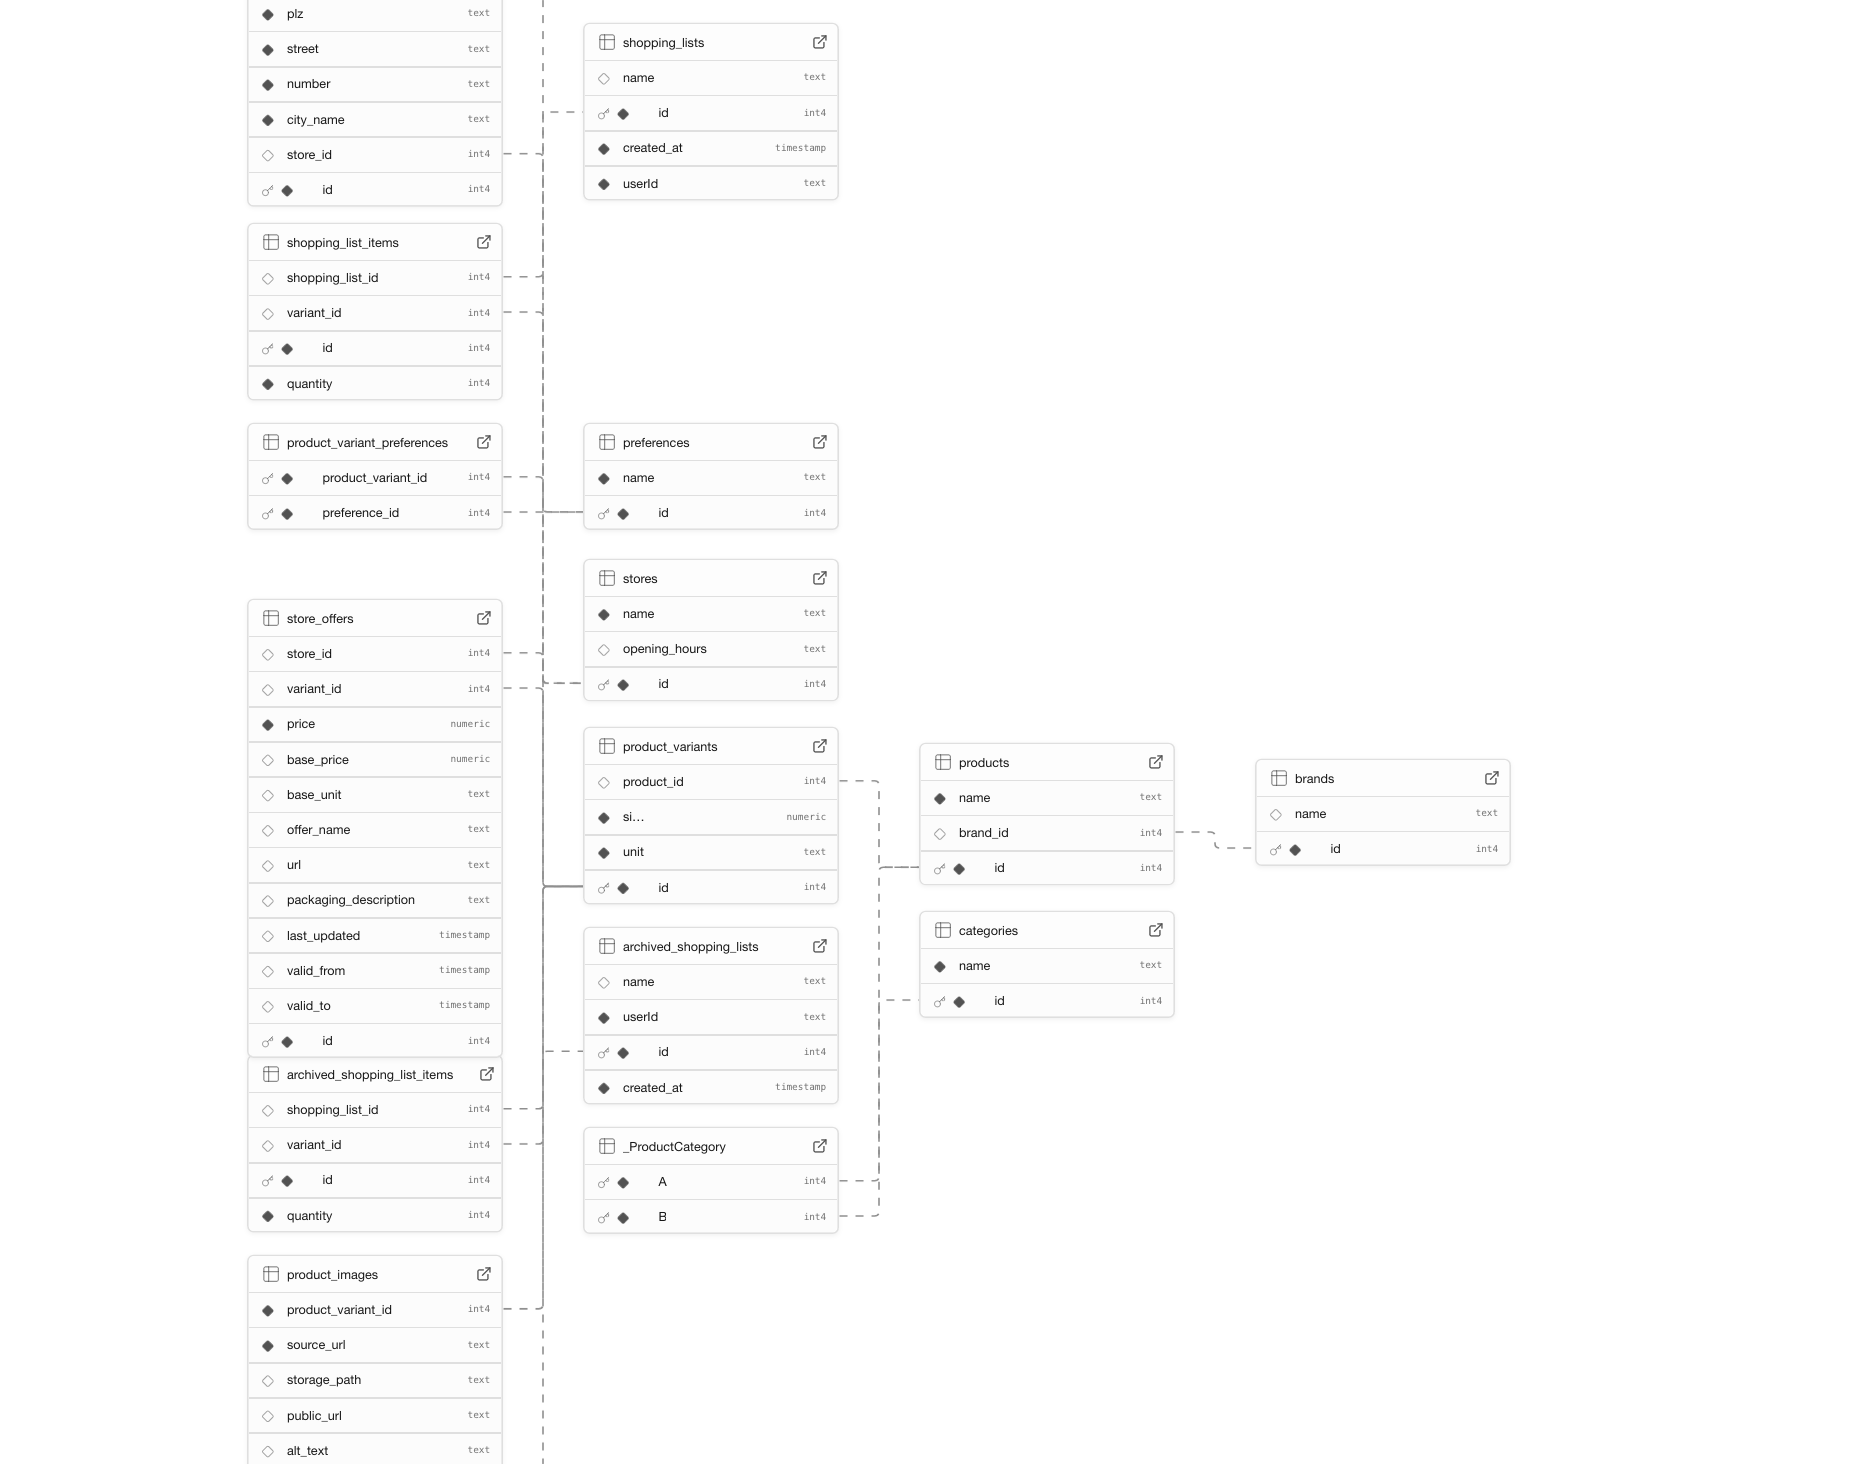
\includegraphics[width=0.98\textwidth]{media/supabase-schema-vgqtxqfvygduzmuwlmba.png}
    \caption{Schematische Übersicht der Projekt-Datenbank (als Supabase-Tabellenmodell)}
    \label{fig:db-schema}
\end{figure}

Die Datenbank vereint folgende Schlüsselaspekte unseres Use Cases:
\begin{itemize}
    \item \textbf{Produktspeicher:} Tabelle \texttt{products} enthält alle eindeutig erkannten Artikel (z.B. „Nutella 750g“), mit Zuordnung zur Marke, logischen Kategorien und beliebig vielen Varianten (\texttt{product\_variants} für Größen, Verpackungseinheiten etc.).
    \item \textbf{Marktübergreifender Vergleich:} Über \texttt{store\_offers} erhält jede Variante je Markt einen eigenen Preissatz – so kann die App tagesaktuell berechnen, welcher Supermarkt für die komplette Einkaufsliste der günstigste ist.
    \item \textbf{Einkaufslistenfunktion:} \texttt{shopping\_lists} und \texttt{shopping\_list\_items} Schnittstellen ermöglichen, nutzerbasierte Listen anzulegen und darin beliebige Produktvarianten in entsprechender Menge zu speichern. So bleibt die Architektur flexibel und beliebig skalierbar.
    \item \textbf{User-Zentrierung:} \texttt{UserId} bei Listen, Präferenzen (\texttt{preferences}), Favoriten, etc. koppelt alle Interaktionen eindeutig an das Anmelde-/Auth-System.
    \item \textbf{Angebots- und Preishistorie:} Über Felder wie \texttt{valid\_from}, \texttt{valid\_to} und \texttt{last\_updated} lassen sich jederzeit Angebotszeitpunkte oder Preisentwicklungen nachvollziehen.
    \item \textbf{Produktbilder und Metadaten:} Die Tabelle \texttt{product\_images} referenziert extern gespeicherte Bilder und bietet so für KI-basierte Such- oder Bilderkennungsideen einen klaren Ankerpunkt.
    \item \textbf{Erweiterbarkeit:} Zusätzliche Features (z.B. Präferenzen, Archiv, Benutzerfavoriten) können einfach durch weitere Tabellen oder Relationen ergänzt werden.
\end{itemize}

\section{Fazit}

Die konsequente Migration auf eine Prisma-verwaltete PostgreSQL-Datenbank erwies sich als zentraler Schritt zu einer robusten, flexiblen und wartungsfreundlichen Backend-Architektur. Für die Anforderungen einer KI-gestützten Smart Shopping App ist dieser Ansatz unverzichtbar: Das exakte, maschinenlesbare Datenmodell ist für Integration, automatisierte Weiterverarbeitung und Entwicklung innovativer Backend- bzw. KI-Features essenziell. Gleichzeitig garantiert die gewählte Architektur Zukunftssicherheit und einfache Erweiterbarkeit für neue Funktionen und Use Cases.


%%%%%%%%%%%%%%%%%%%%%%%%%%%%%%%%%%%%%
% DESIGNPHILOSOPHIE
%%%%%%%%%%%%%%%%%%%%%%%%%%%%%%%%%%%%%
\chapter{Designphilosophie und Gestaltungskonzept}
\renewcommand{\authorinitials}{FK}

\section{Überblick}

Die Designphilosophie unserer App orientiert sich stark an einem ganzheitlichen Nutzererlebnis. Ziel war es nicht nur, funktionale Anforderungen zu erfüllen, sondern eine emotionale, intuitive und visuell konsistente Oberfläche zu schaffen. Im Zentrum steht dabei die Analogie zum analogen Einkaufszettel – diese durchzieht das UI-Design sowohl visuell als auch strukturell.

\section{Gestalterische Prinzipien}

Unsere gestalterischen Leitlinien greifen gezielt ineinander, um eine schlüssige Nutzererfahrung mit klarer visueller Identität zu schaffen. Den Ausgangspunkt bildet dabei die bewusste Entscheidung für eine \textbf{Zettel-Optik}, die sich durch runde, schattenwerfende Container und eine helle, zurückhaltende Farbgebung manifestiert. Diese Analogie zum klassischen Einkaufszettel unterstützt nicht nur die Orientierung, sondern verleiht der App auch einen vertrauten Charakter.

Diese visuelle Idee wird durch \textbf{typografische Konsistenz} verstärkt. Einheitliche Schriftarten, Größen und Farben – insbesondere die klar lesbare Schriftart \texttt{SpaceMono} – sorgen für Wiedererkennung und stärken die visuelle Ruhe des Interfaces. Damit Inhalte wie Produktinformationen und Preise im Vordergrund bleiben, wurde gezielt auf dekorative oder überfrachtete UI-Elemente verzichtet.

Ein zentrales Mittel zur Aufrechterhaltung dieser Gestaltung ist die konsequente Verwendung von \texttt{ScrollViews} mit identischem Aufbau in jedem Screen. Diese einheitliche Scrollstruktur vermittelt ein Gefühl der Kohärenz im Navigationsverhalten, unabhängig davon, ob der Nutzer sich auf der Home-Seite, im Archiv oder im Detailbereich befindet.

\section{Modularität und Komponentenstrategie}

Zur Unterstützung der Wartbarkeit und Konsistenz setzen wir auf \textbf{modular aufgebaute, wiederverwendbare UI-Komponenten}. Beispiele hierfür sind:

\begin{itemize}
    \item \texttt{Card}
    \item \texttt{ShoppingListItem}
    \item \texttt{ButtonSquare}
\end{itemize}

Diese Bausteine folgen denselben Designrichtlinien und ermöglichen es, neue Screens mit minimalem Gestaltungsaufwand in das Gesamtdesign zu integrieren.

\section{Interaktion und Mikroanimationen}

Für gezielte Interaktionsführung sorgen dezente Animationen – etwa das Ein- und Ausblenden von Bedienelementen bei Scrollbewegungen. Diese wurden mithilfe von \texttt{react-native-reanimated} umgesetzt. In Kombination mit klaren \textbf{farblichen Kontrasten} für Buttons und Icons entstehen aufgeräumte, strukturierte Layouts, in denen Nutzer schnell erkennen, wo und wie sie interagieren können.

Auch Details wurden sorgfältig bedacht: Alle verwendeten Icons stammen aus der \texttt{Lucide}-Bibliothek und erscheinen in einheitlicher Größe und Stärke. Interaktive Elemente wurden zudem so gestaltet, dass sie den üblichen Anforderungen an \textbf{Touchzielgrößen} auf mobilen Geräten entsprechen.

\section{Fazit}

All diese Prinzipien zahlen auf ein übergeordnetes Ziel ein: ein \textbf{minimalistisches Design}, das die Produkte und Inhalte – also den eigentlichen Zweck der App – in den Mittelpunkt stellt, ohne durch unnötige visuelle Elemente abzulenken.
  

%%%%%%%%%%%%%%%%%%%%%%%%%%%%%%%%%%%%%
% UI-KAPITEL
%%%%%%%%%%%%%%%%%%%%%%%%%%%%%%%%%%%%%
\chapter{Benutzeroberfläche (UI)}
\renewcommand{\authorinitials}{NK}
\label{chap:ui}

\section{Einleitung}
Die Benutzeroberfläche stellt die Verbindung zwischen Nutzer:innen und den technischen Funktionalitäten der Smart Shopping App her. Sie spielt eine zentrale Rolle bei der täglichen Nutzung der App, da sie das Hinzufügen von Produkten zur Einkaufsliste, das Anzeigen und Bearbeiten der Listen sowie die Darstellung der Preisinformationen und Marktvergleiche ermöglicht.

\section{Mockups und zentrale Ansichten}
% Hier können später Skizzen/Mobile Screenshots oder Diagramme eingefügt werden.
% Beispiel (mit Platzhalter):
\begin{figure}[h!]
    \centering
    \fbox{
        \parbox{0.85\textwidth}{
            \vspace{3cm}
            \begin{center}
                \textbf{Abb. 1: Mockup Startansicht der App}\\
                \emph{(Platzhalter für spätere Screenshots oder Entwürfe)}
            \end{center}
            \vspace{3cm}
        }
    }
    \caption{Mockup: Hauptansicht der Smart Shopping App}
    \label{fig:ui_mockup}
\end{figure}

\section{Home-Screen}
\label{sec:home_screen}

\subsection{Nutzerperspektive}

\subsubsection{Zweck des Screens}
Der Home-Screen dient als zentrale Übersicht für die Einkaufsliste des Nutzers und stellt den wichtigsten Interaktionspunkt der Anwendung dar. Hier kann der Nutzer seine aktuelle Einkaufsliste einsehen und einzelne Produkte aus der Liste entfernen. Darüber hinaus besteht die Möglichkeit, die gesamte Liste zu archivieren oder eine neue Einkaufsliste anzulegen, falls noch keine existiert. Der Screen zeigt außerdem den Gesamtpreis der Liste an und ermöglicht den direkten Wechsel zur Detailansicht der Liste.

\subsubsection{UI/UX-Beschreibung}

\textbf{Wichtige UI-Elemente:}
\begin{itemize}
    \item \textbf{TopBar:} Navigationsleiste am oberen Rand
    \item \textbf{ScrollView:} Zeigt die Einkaufsliste als scrollbare Kartenansicht
    \item \textbf{Card-Komponenten:} Jede Karte repräsentiert ein Produkt mit Name, Marke, Menge, Preis, Bild und Lösch-Button
    \item \textbf{ButtonSquare:} Button zum Wechsel in die Detailansicht der Liste
    \item \textbf{Floating View:} Zeigt den Gesamtpreis der Liste an
    \item \textbf{"Create Shopping List"-Button:} Erscheint, wenn noch keine Liste existiert
\end{itemize}

\noindent\textbf{Interaktive Elemente:}
Die Benutzerinteraktion erfolgt über verschiedene gut erreichbare Elemente. Produkte können über den Lösch-Button auf jeder Produktkarte entfernt werden, während die gesamte Einkaufsliste über einen entsprechenden Button archiviert werden kann. Das Anlegen neuer Listen erfolgt über den "Create Shopping List"-Button, und der Wechsel zur Detailansicht ist über den Button mit Einkaufswagen-Icon möglich.

\subsubsection{User Flow}

\textbf{Von welchem Screen kommt der Nutzer hierher?}
Der Nutzer gelangt meistens über die Tab-Navigation als Startscreen oder nach dem Login auf den Home-Screen.

\noindent\textbf{Wohin geht es von hier aus?}
Vom Home-Screen aus stehen dem Nutzer verschiedene Navigationsmöglichkeiten zur Verfügung. Er kann zur Detailansicht der Einkaufsliste wechseln, indem er die entsprechende Option auswählt. Darüber hinaus besteht die Möglichkeit, zu Produktdetails zu navigieren, sofern diese Funktionalität über die Produktkarten implementiert ist. Weitere Optionen umfassen das Archivieren der aktuellen Liste oder das Anlegen einer neuen Liste.

\subsection{Technische Perspektive}

\subsubsection{Code-Architektur}

\textbf{Komponenten:}
\begin{itemize}
    \item ListScreen (Hauptkomponente)
    \item TopBar (Navigationsleiste)
    \item Card (Produktkarte)
    \item ButtonSquare (Floating Action Button)
    \item LoadingSpinner (Ladeanzeige)
\end{itemize}

\noindent\textbf{State Management:}
\begin{itemize}
    \item React State (useState, useEffect, useCallback)
    \item Kontext: useProductContext für Produktdaten und Ladezustand
\end{itemize}

\noindent\textbf{Services/APIs:}
Die Kommunikation mit dem Backend erfolgt über den api-Service, der alle Backend-Requests abwickelt. Dieser umfasst Funktionen wie getShoppingListItems zum Abrufen der Listenelemente, createShoppingList zum Erstellen neuer Listen, deleteFromShoppingList zum Entfernen von Produkten und archiveShoppingList zum Archivieren von Listen.

\subsubsection{Wichtige Funktionen/Methoden}
\begin{itemize}
    \item \textbf{loadList:} Lädt die aktuelle Einkaufsliste und prüft, ob eine existiert.
    \item \textbf{handleCreateShoppingList:} Erstellt eine neue Einkaufsliste via API.
    \item \textbf{handleDelete:} Löscht ein Produkt aus der Liste.
    \item \textbf{handleArchiveList:} Archiviert die aktuelle Liste.
    \item \textbf{calculateTotal:} Berechnet den Gesamtpreis der Einkaufsliste.
    \item \textbf{Scroll-Handling:} Zeigt/Versteckt Floating Buttons je nach Scrollposition (Performance-Optimierung mit react-native-reanimated).
\end{itemize}

\subsubsection{Besondere Herausforderungen}
Bei der Entwicklung des Home-Screens entstanden verschiedene technische Herausforderungen, die spezielle Lösungsansätze erforderten. Die Performance-Optimierung wurde durch den Einsatz von Reanimated für die Animation der Floating Buttons erreicht, um ein flüssiges Benutzererlebnis zu gewährleisten. Eine umfangreiche Fehlerbehandlung mit Alerts und Fallbacks stellt sicher, dass die Anwendung auch bei fehlgeschlagenen API-Requests stabil funktioniert.

Ein besonderer Fokus lag auf der User Experience, wobei unterschiedliche UI-Zustände wie das Fehlen einer Liste, eine leere Liste oder eine gefüllte Liste klar unterschieden und dem Nutzer verständlich kommuniziert werden. Die Synchronisation der Daten wird durch das automatische Neuladen der Liste bei jedem Fokus auf den Screen mittels useFocusEffect gewährleistet, sodass immer die aktuellsten Daten angezeigt werden.

\section{Explore-Screen}
\label{sec:explore_screen}

\subsection{Nutzerperspektive}

\subsubsection{Zweck des Screens}
Der Explore-Screen dient dazu, dem Nutzer eine strukturierte Übersicht über Produktkategorien und verfügbare Supermärkte zu bieten. Dieser Screen ermöglicht es dem Nutzer, gezielt nach Produkten zu suchen, verschiedene Kategorien zu durchstöbern oder Angebote von bestimmten Märkten anzeigen zu lassen. Dadurch wird eine intuitive Navigation durch das gesamte Produktsortiment der App gewährleistet.

\subsubsection{UI/UX-Beschreibung}

\textbf{Zentrale Elemente:}
\begin{itemize}
    \item Oben befindet sich eine Navigationsleiste (TopBar).
    \item Ein prominenter Button ('Add Products') ermöglicht die Produktsuche.
    \item Darunter werden die Lieblingskategorien ('Your Favourites') angezeigt.
    \item Es folgt eine Liste von Kategorien (z.B. Gemüse, Obst, Milch).
    \item Am unteren Ende werden verfügbare Stores (Supermärkte) als auswählbare Felder angezeigt, farblich hervorgehoben je nach Markt.
\end{itemize}

\noindent\textbf{Interaktive Elemente:}
Die Benutzerinteraktion erfolgt über zwei Hauptkategorien von Elementen. Der 'Add Products'-Button öffnet die Produktsuche und ermöglicht den direkten Einstieg in die Produktauswahl. Zusätzlich sind sowohl Kategorien als auch Stores als anklickbare Elemente gestaltet, die zu einer gefilterten Produktsuche führen und dem Nutzer eine zielgerichtete Navigation ermöglichen.

\subsubsection{User Flow}

\textbf{Einstieg:} Der Nutzer gelangt meist von einem Tab-Menü oder der Hauptnavigation auf diesen Screen.

\noindent\textbf{Von hier aus kann der Nutzer:}
Der Explore-Screen bietet verschiedene Navigationsmöglichkeiten für den Nutzer. Über den "Add Products"-Button kann er direkt zur Produktsuche navigieren und mit der Zusammenstellung seiner Einkaufsliste beginnen. Alternativ kann er über eine Kategorie oder einen Store gezielt Produkte filtern und anzeigen lassen, um spezifische Angebote zu finden. Nach der Auswahl wird der Nutzer zur Such- oder Produktübersicht weitergeleitet, wo er seine Auswahl verfeinern kann.

\subsection{Technische Perspektive}

\subsubsection{Code-Architektur}

\textbf{Hauptkomponente:} explore (React Functional Component)

\noindent\textbf{Eingesetzte Komponenten:}
\begin{itemize}
    \item TopBar (Navigation)
    \item SearchButton (Produktsuche)
    \item CategorieField (Favoriten)
    \item CategorieGroup (Kategorien \& Stores)
\end{itemize}

\noindent\textbf{Datenmodell:} Store-Typ aus den globalen Typen

\noindent\textbf{API:} Daten werden über api.getStores() geladen

\noindent\textbf{State Management:} React useState/useEffect (lokaler State)

\subsubsection{Wichtige Funktionen/Methoden}

\begin{itemize}
    \item \textbf{getStoreColor(name: string):} Weist jedem Store eine spezifische Farbe zu.
    \item \textbf{useEffect + fetchStores:} Lädt beim ersten Rendern die Store-Liste asynchron von der API und speichert sie im State.
    \item \textbf{Interaktive Elemente (onPress):} Navigieren mit router.push zur Suchseite, ggf. mit Store-Filter.
\end{itemize}

\subsubsection{Besondere Herausforderungen}
Die Entwicklung des Explore-Screens brachte verschiedene technische Herausforderungen mit sich. Das dynamische Laden und Anzeigen der Stores mit individueller Farbcodierung erforderte eine flexible Architektur, die eine einheitliche Darstellung bei unterschiedlichen Datenquellen gewährleistet. Eine robuste Fehlerbehandlung beim Laden der Stores wurde implementiert, die dem Nutzer mittels Alert-Nachrichten bei Problemen entsprechendes Feedback gibt. Zusätzlich stellte die Gestaltung einer übersichtlichen und intuitiven Benutzeroberfläche trotz der vielen Auswahlmöglichkeiten eine besondere Herausforderung dar, die durch eine durchdachte Kategorisierung und visuelle Hierarchie gelöst wurde.

\section{Search-Screen}
\label{sec:search_screen}

\subsection{Nutzerperspektive}

\subsubsection{Zweck des Screens}
Der Search-Screen ermöglicht es dem Nutzer, gezielt nach Produkten zu suchen, verschiedene Filter anzuwenden und gefundene Produkte zur Einkaufsliste hinzuzufügen. Das Hauptziel besteht darin, eine schnelle und komfortable Möglichkeit zu bieten, passende Angebote zu finden und die Produktauswahl durch Filter für Kategorie und Store zu verfeinern. Dieser Screen stellt somit das Herzstück der Produktsuche und -auswahl dar.

\subsubsection{UI/UX-Beschreibung}

\textbf{Zentrale Elemente:}
\begin{itemize}
    \item \textbf{Suchleiste:} Oben mittig, ermöglicht die Suche nach Produktnamen oder Marken.
    \item \textbf{Filter-Button:} Links neben der Suchleiste öffnet ein Modal für Filteroptionen (Kategorie, Store).
    \item \textbf{Cancel-Button:} Rechts neben der Suchleiste, löscht die aktuelle Suche.
    \item \textbf{Produktliste:} Zeigt gefilterte oder alle Produkte als Karten an, sortiert nach günstigstem Preis.
    \item \textbf{Produktkarte:} Enthält Produktdetails und einen Button (PlusCircle), um das Produkt zur Einkaufsliste hinzuzufügen.
    \item \textbf{Filter-Modal:} Ermöglicht Mehrfachauswahl von Kategorien und Stores, sowie das Zurücksetzen oder Anwenden der Filter.
    \item \textbf{Ladespinner:} Wird angezeigt, solange die Produktdaten geladen werden.
\end{itemize}

\noindent\textbf{Interaktive Elemente:}
Der Search-Screen bietet dem Nutzer verschiedene Interaktionsmöglichkeiten für eine effiziente Produktsuche. Die Suchleiste als Textinput ermöglicht die direkte Eingabe von Suchbegriffen, während der Filter-Button ein Modal mit erweiterten Filteroptionen öffnet. Ein Cancel-Button setzt die aktuelle Suche zurück und ermöglicht einen Neustart. Die Produktkarten sind klickbar und führen zur Detailansicht der jeweiligen Artikel. Der PlusCircle-Button auf jeder Karte fügt das entsprechende Produkt direkt zur Einkaufsliste hinzu. Das Filter-Modal selbst enthält MultiSelects für die Auswahl sowie Reset- und Apply-Buttons für die Filterverwaltung.

\subsubsection{User Flow}
\textbf{Einstieg:} Der Nutzer gelangt meist von einem Tab oder durch Auswahl eines Stores auf den Search-Screen.

\noindent\textbf{Aktionen:} Auf diesem Screen kann der Nutzer verschiedene Aktionen durchführen, um seine Produktsuche zu optimieren. Er kann gezielt nach Produkten suchen, verschiedene Filter anwenden, gefundene Produkte direkt zur Einkaufsliste hinzufügen oder detaillierte Produktinformationen aufrufen.

\noindent\textbf{Navigation:}
Die Navigation vom Search-Screen aus bietet verschiedene Möglichkeiten. Ein Klick auf ein Produkt führt zur Detailansicht, während das Anwenden von Filtern eine aktualisierte Produktliste zur Verfügung stellt. Darüber hinaus ist die Rückkehr zu anderen Tabs oder Screens jederzeit möglich, um einen flexiblen Workflow zu gewährleisten.

\subsection{Technische Perspektive}

\subsubsection{Code-Architektur}

\textbf{Hauptkomponente:} SearchSite (funktionale React-Komponente)

\noindent\textbf{Verwendete Komponenten:}
\begin{itemize}
    \item SearchBar (benutzerdefinierte Suchleiste)
    \item CustomMultiSelect (Filterauswahl)
    \item SearchCard (Produktkarte)
    \item ButtonSizeable, ButtonTransparent (Buttons)
    \item LoadingSpinner (Ladesymbol)
\end{itemize}

\noindent\textbf{State Management:} React Context (useProductContext) für Produkte und Laden-Status

\noindent\textbf{API:} Zugriff auf Stores und Produkte über api-Service

\subsubsection{Abhängigkeiten}

\textbf{Services:} api (z.B. getStores, addToShoppingList)

\noindent\textbf{State:} Produkte, Stores, Filterauswahl, Suchbegriff, Ladezustand

\noindent\textbf{Libraries:} expo-router, @shopify/flash-list, lucide-react-native (Icons), React Native Komponenten

\subsubsection{Wichtige Funktionen/Methoden}
\begin{itemize}
    \item \textbf{handleSearch(query):} Filtert Produkte nach Suchbegriff und sortiert nach Preis.
    \item \textbf{applyFilters():} Wendet Suchbegriff, Kategorie- und Store-Filter an, sortiert Ergebnis.
    \item \textbf{fetchStores():} Holt Store-Daten von der API.
    \item \textbf{useEffect-Hooks:}
    \begin{itemize}
        \item Lädt Stores beim Mounten.
        \item Setzt Store-Filter, wenn ein Store-Name als Parameter übergeben wird.
        \item Lädt Produkte, falls noch nicht vorhanden.
        \item Wendet Filter automatisch an, wenn sich die Store-Auswahl ändert.
    \end{itemize}
    \item \textbf{renderItem:} Rendert einzelne Produktkarten mit Interaktionsmöglichkeiten.
\end{itemize}

\subsubsection{Besondere Herausforderungen}
Die Entwicklung des Search-Screens stellte verschiedene komplexe Herausforderungen dar, die innovative Lösungsansätze erforderten. Die Implementierung der Filterlogik erwies sich als besonders anspruchsvoll, da eine Kombination aus Suchbegriff, Kategorie- und Store-Filter inklusive intelligenter Sortierung realisiert werden musste. Für die Performance-Optimierung wurde FlashList eingesetzt, um auch bei großen Produktlisten ein performantes Rendering zu gewährleisten.

Die State-Synchronisation stellte eine weitere Herausforderung dar, da Filter automatisch bei Änderung der Auswahl angewendet und gleichzeitig mit dem globalen Context synchronisiert werden müssen. Besondere Aufmerksamkeit galt auch der User Experience, wobei eine durchdachte Reset- und Apply-Logik im Filter-Modal implementiert wurde, die dem Nutzer sofortige Rückmeldung bei Suche und Filterung bietet.

\section{UI-Komponenten}
\label{sec:ui_komponenten}

\subsection{Home(index)}

\subsubsection{Card}

\noindent\textbf{Aufbau und Funktionsweise:}
Die Card-Komponente ist eine React Native-Komponente, die die Daten eines einzelnen Produkts als Karte darstellt. Sie erhält alle relevanten Produktinformationen (Name, Marke, Größe, Einheit, Preis, Menge, Bild-URL) sowie optionale Callback-Funktionen für das Auswählen (onPress) und Löschen (onDelete). Die Komponente nutzt einen Swipeable-Container, um die Löschfunktion per Wischgeste zu ermöglichen.

\noindent\textbf{Darstellung:}
Das Produkt wird in einer horizontalen Karte angezeigt. Links befindet sich das Produktbild, daneben die Produktdetails wie Name, Marke, Größe, Einheit und Preis. Die Menge wird, falls vorhanden, ganz rechts angezeigt. Die Karte ist optisch ansprechend gestaltet, mit abgerundeten Ecken, Schatten und modernen Farben.

\noindent\textbf{Interaktive Elemente:}
Die Karte kann angetippt werden, um eine Aktion auszulösen (z.\,B. Details anzeigen), sofern eine onPress-Funktion übergeben wurde. Durch Wischen nach links erscheint ein rotes Feld mit einem Papierkorb-Icon, über das das Produkt gelöscht werden kann. Die Löschfunktion wird nur angezeigt, wenn eine onDelete-Funktion vorhanden ist.

\noindent\textbf{Verwendung:}
Die Card-Komponente wird innerhalb von Produktlisten eingesetzt, um einzelne Produkte übersichtlich und interaktiv darzustellen. Sie eignet sich besonders für Einkaufslisten oder Produktübersichten, bei denen Nutzer Produkte auswählen oder entfernen können. Die Komponente ist flexibel und kann in verschiedenen Kontexten wiederverwendet werden.

\subsection{Explore}

\subsubsection{CategorieField}
Die Komponente CategorieField ist ein wiederverwendbares React Native-UI-Element, das eine Kategorie als anklickbares Feld darstellt. Sie nimmt folgende Props entgegen:
\begin{itemize}
    \item \textbf{title:} Der Name der Kategorie (wird als Text angezeigt).
    \item \textbf{image:} Optionales Bild, das dekorativ rechts oben im Feld angezeigt wird.
    \item \textbf{backgroundColor:} Optionaler Hintergrundfarbwert (Standard: "\#4B946A").
    \item \textbf{onPress:} Optionaler Callback, der beim Antippen des Feldes ausgeführt wird.
\end{itemize}

\noindent\textbf{Aufbau:}
Das Haupt-Element basiert auf einem Pressable, das das gesamte Feld anklickbar macht und eine intuitive Benutzerinteraktion ermöglicht. Im Feld wird der Titel als weißer, fetter Text oben links angezeigt, was eine gute Lesbarkeit gewährleistet. Falls ein Bild übergeben wird, erscheint es dekorativ rechts oben, leicht gedreht und abgerundet, was dem Design eine moderne Note verleiht. Das Layout nutzt Tailwind-Klassen und Style-Props für ein responsives und modernes Design, das sich an verschiedene Bildschirmgrößen anpasst.

\noindent\textbf{Verwendung:} Die Komponente eignet sich hervorragend, um Kategorien in einer Übersicht darzustellen, beispielsweise in einer Liste oder einem Grid-Layout. Sie kann individuell mit Titel, Bild und Farbe angepasst und mit einer spezifischen Aktion beim Klick versehen werden, was eine hohe Flexibilität in der Anwendung ermöglicht.

\subsubsection{CategorieGroup}
Die Komponente CategorieGroup dient dazu, eine Gruppe von Kategorien als übersichtliche, responsive Felder darzustellen. Sie nimmt ein Array von Kategorien entgegen und ordnet diese in Reihen mit jeweils zwei Feldern an. Bei einer ungeraden Anzahl wird das erste Feld einzeln in einer eigenen Reihe angezeigt.

\noindent\textbf{Aufbau und Funktionsweise:}

\textbf{Props:}
\begin{itemize}
    \item \textbf{categories:} Ein Array von Kategorie-Objekten mit Titel, Bild, Hintergrundfarbe und -optionaler Aktion.
    \item \textbf{onPress:} Optionaler Callback, der beim Klick auf ein Feld ausgeführt wird und die jeweilige Kategorie übergibt.
\end{itemize}

\textbf{Logik:}
Die Komponente führt zunächst eine Überprüfung durch, ob Kategorien vorhanden sind, bevor sie mit der Darstellung beginnt. Bei einer ungeraden Anzahl von Kategorien wird das erste Element einzeln angezeigt, während die restlichen Kategorien paarweise gruppiert werden. Jede Reihe wird als View mit zwei Feldern (CategorieField) dargestellt, wobei unvollständige Reihen mit einem leeren Feld aufgefüllt werden, um ein konsistentes Layout zu gewährleisten.

\textbf{Layout:}
Das Design nutzt Flexbox und Tailwind-Klassen für ein modernes, flexibles Layout, das sich verschiedenen Bildschirmgrößen anpasst. Die Felder sind gleichmäßig verteilt und haben definierte Abstände zwischen den Reihen, was eine ansprechende visuelle Hierarchie schafft.

\noindent\textbf{Verwendung:} CategorieGroup eignet sich optimal, um Kategorien in einer übersichtlichen, klickbaren Grid-Ansicht darzustellen, beispielsweise auf einer Explore-Seite. Die Komponente ist flexibel gestaltet und kann individuell mit verschiedenen Aktionen und Design-Optionen erweitert werden, um spezifische Anforderungen zu erfüllen.

\subsubsection{SearchButton}
Die Komponente SearchButton ist ein klickbarer Button, der wie ein Suchfeld aussieht, aber kein Eingabefeld ist. Sie zeigt ein Lupen-Icon und einen beschrifteten Text (Standard: "Add Products") an.

\noindent\textbf{Aufbau:}

\textbf{Props:}
\begin{itemize}
    \item \textbf{label:} Optionaler Text, der im Button angezeigt wird.
    \item \textbf{onPress:} Optionaler Callback, der beim Klick ausgeführt wird.
\end{itemize}

\textbf{Darstellung:}
Die Komponente basiert auf einem Pressable mit abgerundeten Ecken, weißem Hintergrund und grauem Rahmen, was ihr ein sauberes und professionelles Aussehen verleiht. Das Lupen-Icon (Search aus lucide-react-native) wird links neben dem Text positioniert und signalisiert dem Nutzer die Suchfunktionalität. Der Button reagiert visuell auf Berührungen durch eine verringerte Opazität und bietet auf Android-Geräten zusätzlich einen Ripple-Effekt für taktiles Feedback.

\noindent\textbf{Verwendung:} SearchButton eignet sich hervorragend als auffälliger, interaktiver Button für Such- oder Hinzufügen-Aktionen, beispielsweise am oberen Rand einer Produktliste. Die Komponente ist einfach anpassbar und kann flexibel überall eingesetzt werden, wo ein solcher funktionaler Button benötigt wird.

\subsubsection{StoreIcons}
Der Ordner icons innerhalb von categories enthält die grafischen Symbole für verschiedene Supermärkte und Einkaufskategorien, die in der App verwendet werden. Jede Icon-Komponente repräsentiert einen bestimmten Markt, wie zum Beispiel Lidl, Aldi oder Rewe, und liegt als eigene Datei im Ordner vor.

Die Datei index.tsx dient als zentrale Sammelstelle für alle Icons. Sie exportiert die einzelnen Komponenten unter einheitlichen Namen, sodass sie in anderen Teilen der Anwendung unkompliziert und übersichtlich importiert werden können. Das erleichtert die Wiederverwendung und sorgt für eine klare Struktur im Code.

Insgesamt ermöglicht dieser Aufbau, dass die Icons konsistent und effizient im Frontend eingesetzt werden können, zum Beispiel zur Visualisierung von Märkten in Listen oder Übersichten. Die zentrale Exportdatei vereinfacht die Verwaltung und trägt zur besseren Wartbarkeit des Projekts bei.

\subsection{Search}

\subsubsection{SearchBar}
Die Komponente SearchBar ist eine interaktive Suchleiste für React Native, die Benutzereingaben entgegennimmt und Suchanfragen auslöst.

\noindent\textbf{Aufbau und Funktionsweise:}

\textbf{Props:}
\begin{itemize}
    \item \textbf{placeholder:} Optionaler Platzhaltertext im Eingabefeld (Standard: "Search...").
    \item \textbf{onSearch:} Callback, der bei jeder Änderung des Suchbegriffs aufgerufen wird.
\end{itemize}

\hangindent=2em
\hangafter=1
\textbf{Ref-API:}
Über das ref kann die Methode clear von außen aufgerufen werden, um das Suchfeld zu leeren und die Tastatur zu schließen.

\textbf{Logik:}
Die Eingabe wird im State query gespeichert und jede Änderung im Textfeld löst den onSearch-Callback mit dem aktuellen Wert aus. Ein Klick auf die Leiste fokussiert das Eingabefeld automatisch, was die Benutzerfreundlichkeit erhöht. Die Methode clearSearch setzt das Feld zurück und schließt die Tastatur, um eine saubere Benutzeroberfläche zu gewährleisten.

\textbf{Darstellung:}
Die Suchleiste besteht aus einem weißen, abgerundeten Container mit einem integrierten TextInput. Das TextInput ist direkt fokussierbar und optisch schlicht gehalten, um die Aufmerksamkeit auf die Eingabe zu lenken.

\noindent\textbf{Verwendung:} SearchBar eignet sich optimal für Suchfunktionen in Listen oder Übersichten. Sie kann von außen gesteuert werden, beispielsweise zum programmatischen Zurücksetzen, und ist flexibel für verschiedene Anwendungsfälle einsetzbar.

\subsubsection{CustomMultiSelect}
Die Komponente CustomMultiSelect ist ein individuell gestaltetes Mehrfach-Auswahlfeld für React Native, basierend auf react-native-element-dropdown. Sie ermöglicht die Auswahl mehrerer Optionen aus einer Liste und bietet eine Suchfunktion.

\noindent\textbf{Aufbau und Funktionsweise:}

\textbf{Props:}
\begin{itemize}
    \item \textbf{data:} Array von Auswahloptionen mit label und value.
    \item \textbf{labelField, valueField:} Feldnamen für Anzeige und Wert.
    \item \textbf{placeholder:} Platzhaltertext im Auswahlfeld.
    \item \textbf{value:} Array der aktuell ausgewählten Werte.
    \item \textbf{onChange:} Callback, der bei Änderung der Auswahl ausgelöst wird.
    \item Diverse Style-Props zur Anpassung des Designs.
    \item \textbf{search:} Aktiviert die Suchfunktion (Standard: true).
    \item \textbf{maxHeight:} Maximale Höhe der Dropdown-Liste.
\end{itemize}

\textbf{Darstellung:}
Die Dropdown-Liste zeigt alle verfügbaren Optionen übersichtlich an, wobei ausgewählte Elemente mit einem Haken-Icon markiert werden. Ausgewählte Items werden als Chips oberhalb der Liste angezeigt und bieten die Möglichkeit zum schnellen Entfernen über ein ×-Symbol. Die Komponente ist optisch anpassbar und nutzt Tailwind-Klassen für ein modernes Design, das sich harmonisch in verschiedene UI-Kontexte einfügt.

\textbf{Logik:}
Die Auswahl und das Entfernen von Items werden vollständig über die Props gesteuert, was eine saubere Datenhaltung gewährleistet. Die integrierte Suchfunktion filtert die angezeigten Optionen in Echtzeit und verbessert die Benutzerfreundlichkeit bei großen Datensätzen.

\noindent\textbf{Verwendung:} CustomMultiSelect eignet sich hervorragend für Filter- und Auswahlfunktionen, bei denen mehrere Werte gleichzeitig gewählt werden können, beispielsweise zur Produktsuche oder Kategoriefilterung. Sie ist flexibel gestaltet und lässt sich einfach in verschiedene UI-Kontexte integrieren.

\subsection{(Produkt-)Details}

\subsubsection{Field}
Die Komponente Field ist ein flexibler, klickbarer Button für React Native, der ein Icon und optional einen Text anzeigt.

\noindent\textbf{Aufbau und Funktionsweise:}

\textbf{Props:}
\begin{itemize}
    \item \textbf{icon:} Das anzuzeigende Icon (React-Komponente).
    \item \textbf{text:} Optionaler Text, der neben dem Icon angezeigt wird.
    \item \textbf{iconColor:} Farbe des Icons (wird über das Icon selbst gesteuert).
    \item \textbf{backgroundColor:} Hintergrundfarbe des Buttons.
    \item \textbf{onPress:} Optionaler Callback, der beim Klick ausgeführt wird.
\end{itemize}

\textbf{Darstellung:}
Der Button präsentiert sich mit abgerundeten Ecken und ist horizontal ausgerichtet und zentriert angeordnet. Das Icon wird links positioniert, während der Text, falls vorhanden, rechts daneben platziert wird. Der Hintergrund ist individuell anpassbar, was eine flexible Gestaltung ermöglicht. Die Klick-Animation wird über activeOpacity gesteuert und bietet dem Nutzer visuelles Feedback bei der Interaktion.

\noindent\textbf{Verwendung:} Field eignet sich für verschiedene Interaktionsmöglichkeiten, beispielsweise als Mengen-Auswahl, Aktions-Button oder für Eingabefelder mit Icon-Unterstützung. Das Design ist flexibel angelegt und kann mit unterschiedlichen Icons, Farben und Texten verwendet werden, um verschiedene Anwendungsfälle abzudecken.

\subsubsection{QuantityInput}
Die Komponente QuantityInput ist ein Eingabefeld für Mengenangaben, das Benutzern ermöglicht, eine Zahl durch Plus- und Minus-Buttons zu erhöhen oder zu verringern.

\noindent\textbf{Aufbau und Funktionsweise:}

\textbf{Props:}
\begin{itemize}
    \item \textbf{value:} Startwert der Menge (Standard: 1).
    \item \textbf{onChange:} Callback, der bei jeder Änderung der Menge ausgelöst wird.
    \item \textbf{min, max:} Minimale und maximale erlaubte Werte (Standard: 1 bis 99).
\end{itemize}

\textbf{Logik:}
Die aktuelle Menge wird im State quantity verwaltet und bietet eine zentrale Kontrolle über den Wert. Beim Klick auf den Minus-Button wird die Menge um eins verringert, solange sie über dem definierten Minimum liegt. Entsprechend wird beim Klick auf den Plus-Button die Menge um eins erhöht, solange sie unter dem festgelegten Maximum bleibt. Jede Änderung löst den onChange-Callback mit dem neuen Wert aus, was eine nahtlose Integration in übergeordnete Komponenten ermöglicht.

\textbf{Darstellung:}
Die Komponente besteht aus einer horizontal angeordneten Reihe mit einem Minus-Button, der zentralen Mengenanzeige und einem Plus-Button. Die Buttons sind rund gestaltet und heben sich optisch deutlich ab, während die aktuelle Menge mittig und gut lesbar angezeigt wird.

\noindent\textbf{Verwendung:} QuantityInput eignet sich optimal für Produktdetailseiten oder Warenkörbe, wo Nutzer die gewünschte Menge eines Artikels präzise einstellen können. Sie ist intuitiv bedienbar und flexibel in verschiedenen Kontexten einsetzbar.

\subsubsection{ProductLoadingSkeleton}
Die Komponente ProductLoadingSkeleton zeigt ein Ladeplatzhalter-Layout für Produktdetailseiten an, während die echten Daten geladen werden.

\noindent\textbf{Aufbau und Funktionsweise:}

\textbf{Darstellung:}
Die Komponente besteht aus mehreren grauen, animierten Rechtecken (``Skeletons''), die die Struktur der später angezeigten Produktinformationen nachahmen und dem Nutzer eine Vorschau auf das kommende Layout bieten. Es sind Platzhalter für das Produktbild, den Titel, Varianten, Angebote und einen Button vorhanden, die alle wichtigen Bereiche der Produktdetailseite abdecken. Die Platzhalter sind mit der Klasse animate-pulse versehen, um eine pulsierende Ladeanimation darzustellen, die Aktivität signalisiert und die Wartezeit angenehmer gestaltet.

\textbf{Layout:}
Die Elemente sind optisch so angeordnet, wie die echten Produktdetails später erscheinen werden, was eine nahtlose Transition gewährleistet. Das Layout ist responsiv gestaltet und zentriert ausgerichtet, um auf verschiedenen Bildschirmgrößen optimal zu funktionieren.

\noindent\textbf{Verwendung:} ProductLoadingSkeleton wird angezeigt, wenn Produktdaten noch nicht vollständig geladen sind, um dem Nutzer visuelles Feedback zu geben und die Wartezeit angenehmer zu gestalten. Sie verbessert die User Experience erheblich durch ein modernes Lade-Design, das Transparenz über den Ladezustand schafft und die wahrgenommene Ladezeit reduziert.

\subsection{Generelle UI-Komponenten}

\subsubsection{NavigationBar(TopBar)}
Die TopBar-Komponente stellt die obere Navigationsleiste der App dar und sorgt für eine konsistente Benutzerführung. Sie nimmt optional einen Titel und die Information entgegen, ob ein Zurück-Button angezeigt werden soll. Ist der Zurück-Button aktiv, kann der Nutzer zur vorherigen Seite zurückkehren. Andernfalls wird das Profilbild des aktuell angemeldeten Nutzers angezeigt, das als Button dient und beim Antippen zu den Einstellungen weiterleitet. Die Komponente verwendet React Native-Elemente für das Layout und Styling sowie Expo Router für die Navigation. Die Benutzerinformationen werden über Clerk eingebunden, sodass das Profilbild dynamisch geladen wird. Das Design ist flexibel und passt sich je nach Kontext an, wodurch die Komponente universell auf verschiedenen Screens eingesetzt werden kann.

\subsubsection{SignOutButton}

\noindent\textbf{Aufbau und Funktionsweise:}
Die SignOutButton-Komponente ist eine React Native-Komponente, die die Abmeldung eines Nutzers aus der App ermöglicht. Sie verwendet das Clerk-Auth-System und ruft beim Klick auf den Button die signOut-Funktion auf. Nach erfolgreichem Logout wird der Nutzer automatisch zur Startseite weitergeleitet. Fehler beim Abmelden werden in der Konsole ausgegeben.

\noindent\textbf{Darstellung:}
Der Button ist horizontal aufgebaut und besteht aus einem roten Logout-Icon sowie dem Text \enquote{Sign out}. Das Design ist modern und passt sich je nach Plattform (iOS oder Android) an, um ein natives Erscheinungsbild zu gewährleisten. Die Farben und abgerundeten Ecken sorgen für eine klare visuelle Trennung.

\noindent\textbf{Interaktive Elemente:}
Das zentrale interaktive Element ist der Button selbst. Ein Klick darauf löst die Abmeldefunktion aus. Die Komponente reagiert auf Touch-Events und gibt visuelles Feedback durch die Gestaltung und Animationen.

\noindent\textbf{Verwendung:}
Die SignOutButton-Komponente wird überall dort eingesetzt, wo Nutzer die Möglichkeit haben sollen, sich aus der App abzumelden, beispielsweise im Profil- oder Einstellungsbereich. Sie sorgt für eine einfache und sichere Abmeldung und kann flexibel in verschiedenen Bereichen der App eingebunden werden.

\subsubsection{ButtonSquare}
Die ButtonSquare-Komponente ist ein quadratischer, interaktiver Button, der in der App als Floating Action Button (FAB) fungiert. Er wird in der Regel am unteren rechten Bildschirmrand platziert und hebt sich durch seine Größe und Form von anderen UI-Elementen ab. Der Button kann mit einem Icon versehen werden, das eine spezifische Aktion repräsentiert, wie beispielsweise das Hinzufügen eines neuen Elements oder das Starten einer Suche. Die Komponente nutzt Pressable für die Interaktivität und bietet visuelles Feedback bei Berührung. Sie ist so gestaltet, dass sie sowohl auf iOS als auch auf Android gut aussieht und funktioniert, und kann leicht in verschiedene Screens integriert werden.

\subsubsection{ButtonSizeable}
Die ButtonSizeable-Komponente ist ein anpassbarer Button, der in der Größe variabel ist und sich somit flexibel in verschiedene Layouts einfügen lässt. Er kann sowohl als runder als auch als quadratischer Button dargestellt werden, je nach den Anforderungen des Designs. Die Größe des Buttons kann über Props gesteuert werden, sodass Entwickler ihn leicht an unterschiedliche Bildschirmgrößen und -auflösungen anpassen können. Die Komponente verwendet ebenfalls Pressable für die Interaktivität und bietet visuelles Feedback bei Berührung. Sie ist so gestaltet, dass sie auf beiden Plattformen, iOS und Android, gut aussieht und funktioniert.

\subsubsection{ButtonTransparent}
Die ButtonTransparent-Komponente ist ein transparenter, klickbarer Button, der in der App verwendet wird, um Aktionen auszulösen, ohne dabei die darunter liegende UI zu verdecken. Er eignet sich ideal für Situationen, in denen eine subtile Interaktion gewünscht ist, beispielsweise in Overlay- oder Modal-Fenstern. Der Button kann mit einem Icon oder Text versehen werden und nutzt Pressable für die Interaktivität. Durch seine Transparenz fügt er sich harmonisch in das Design ein und ermöglicht es dem Nutzer, Aktionen auszuführen, ohne die visuelle Klarheit der App zu beeinträchtigen.

\subsubsection{ButtonRound}
Die ButtonRound-Komponente ist ein runder, interaktiver Button, der in der App verwendet wird, um Aktionen auszulösen. Er eignet sich besonders gut für Situationen, in denen ein auffälliges, zentrales Element benötigt wird, beispielsweise für das Starten einer neuen Aktion oder das Hinzufügen eines neuen Elements. Der Button kann mit einem Icon oder Text versehen werden und nutzt Pressable für die Interaktivität. Durch seine runde Form hebt er sich von anderen UI-Elementen ab und zieht die Aufmerksamkeit des Nutzers auf sich.

\vspace{1em}
\noindent
Dieses Kapitel liefert einen Rahmen für die Dokumentation der Benutzeroberfläche und kann im Laufe des Projekts kontinuierlich mit Inhalten, Screenshots und technischen Details erweitert werden.




\chapter{Benutzerverwaltung und Personalisierung}
\renewcommand{\authorinitials}{FK}
%%%%%%%%%%%%%%%%%%%%%%%%%%%%%%%%%%%%%
% LOGIN & SIGN-UP
%%%%%%%%%%%%%%%%%%%%%%%%%%%%%%%%%%%%%
\section{Login- und Registrierungsfunktion}

\subsection{Nutzerperspektive}

Die Login- und Registrierungsseiten ermöglichen einen klar geführten Einstieg in die App – sowohl über moderne Single-Sign-On-Methoden (Google, Apple) als auch über die klassische Kombination aus E-Mail und Passwort. Unabhängig vom gewählten Weg erfolgt die gesamte Authentifizierung über den integrierten Dienst \texttt{Clerk}, der eine sichere Verwaltung aller Nutzerdaten übernimmt.

Beim Sign-Up gibt der Nutzer zunächst seinen Namen, seine E-Mail-Adresse und ein Passwort an. Danach wird automatisch ein Verifizierungscode per E-Mail versendet, der zur Aktivierung des Kontos eingegeben werden muss. Erst nach erfolgreicher Verifikation wird der Zugang freigeschaltet.

Auch der Login mit E-Mail und Passwort ist vollständig implementiert – inklusive Sessionhandling und sicherem Redirect zur Startseite nach erfolgreicher Anmeldung. Alternativ kann sich der Nutzer direkt per Google- oder Apple-Konto authentifizieren. Die entsprechenden Optionen sind prominent und visuell getrennt dargestellt, was für Klarheit sorgt.

Die gesamte Nutzeroberfläche ist durchgängig strukturiert – mit Icons zur Passwortanzeige, deutlicher Trennung der Authentifizierungsarten und flüssiger Navigation zwischen Anmelde- und Registrierungsprozess. Egal ob klassisch oder via SSO – nach erfolgreichem Login landet der Nutzer direkt auf der Startseite der App.

\subsection{Technische Perspektive}

Die technische Architektur basiert auf klassischen \texttt{React Native}-Komponenten wie \texttt{KeyboardAvoidingView}, \texttt{ScrollView}, \texttt{TextInput} und \texttt{TouchableOpacity}, ergänzt durch \texttt{Ionicons} für visuelles Feedback. Als Authentifizierungsdienst kommt \texttt{Clerk} zum Einsatz – über Hooks wie \texttt{useSignIn}, \texttt{useSignUp} und \texttt{useSSO}. Für OAuth werden \texttt{expo-auth-session} und \texttt{WebBrowser} verwendet.

Die Zustände werden lokal mit \texttt{useState}, \texttt{useEffect} und \texttt{useCallback} verwaltet. Die wichtigsten Funktionen sind:

\begin{itemize}
    \item \texttt{onSignInPress()} – für den klassischen Login mit E-Mail/Passwort
    \item \texttt{onSignUpPress()} – für die Registrierung inkl. Start der E-Mail-Verifikation
    \item \texttt{onVerifyPress()} – zur Eingabe und Prüfung des E-Mail-Codes
    \item \texttt{onGooglePress()}, \texttt{onApplePress()} – starten den jeweiligen OAuth-Flow
    \item \texttt{useWarmUpBrowser()} – initialisiert den Webbrowser vorab zur Beschleunigung des OAuth-Flows
\end{itemize}

Herausfordernd ist die saubere Trennung der Logik für die beiden Authentifizierungswege (klassisch vs. OAuth) sowie die Absicherung gegen unvollständige Eingaben. Auch das Sessionhandling und das asynchrone Verhalten müssen korrekt auf den UI-State abgebildet werden. Die Eingabefelder wurden zudem so integriert, dass sie insbesondere auf iOS gerätefreundlich mit der Tastatur interagieren.


%HomeScreen
%search
%%%%%%%%%%%%%%%%%%%%%%%%%%%%%%%%%%%%%
% SETTINGS-SCREEN
%%%%%%%%%%%%%%%%%%%%%%%%%%%%%%%%%%%%%
\chapter{Einstellungen und Nutzerprofil}
\renewcommand{\authorinitials}{FK}

\section{Nutzerperspektive}

Der Einstellungen-Screen stellt eine zentrale Steuerzentrale für den Nutzer dar. Hier kann er seine Profildaten einsehen, auf Hilfeseiten zugreifen, zu archivierten Listen oder zur Einkaufsliste navigieren oder sich aus der App ausloggen.

Gestalterisch ist der Screen in mehrere klar voneinander abgegrenzte Bereiche unterteilt: ein Profilbereich, die eigentlichen Einstellungseinträge, ein Support-Block und der Logout-Bereich. Im oberen Bereich befindet sich das runde Profilbild des Nutzers, ergänzt durch Name und E-Mail-Adresse, sowie ein Chevron-Icon, das auf Interaktivität hinweist.

Darunter folgen mehrere Einstellungseinträge in Form von \texttt{SettingsRows}, die jeweils mit einem Icon, einem Titel und ggf. einem Untertitel versehen sind. Diese werden visuell voneinander getrennt durch weiße Hintergründe, Schatten und abgerundete Kanten. Ein durchgängiges Icon-Design sorgt für visuelle Konsistenz.

Der User Flow ist einfach: Der Nutzer gelangt über den Bottom Tab \enquote{Settings} zum Screen. Von dort kann er durch Antippen seines Profils das \texttt{UserProfile}-Modal von \texttt{Clerk} öffnen, zum Archiv navigieren oder sich abmelden. Einträge wie \enquote{Shopping Lists} oder \enquote{Support} sind aktuell noch nicht mit konkreter Funktion hinterlegt.

\section{Technische Perspektive}

Die Hauptkomponente \texttt{SettingsScreen} wird ergänzt durch die beiden Subkomponenten \texttt{SettingsGroup} (als Wrapper für gruppierte Einträge) und \texttt{SettingsRow} (für einzelne Einstellungen). Ergänzt wird dies durch die \texttt{TopBar} sowie den \texttt{SignOutButton}.

Die wichtigsten Abhängigkeiten umfassen:

\begin{itemize}
    \item \texttt{@clerk/clerk-expo} – für Benutzerinformationen und Sessionhandling
    \item \texttt{lucide-react-native} – für einheitliche Icons
    \item \texttt{expo-router} – zur Navigation zwischen den Screens
    \item klassische \texttt{React Native}-Komponenten – für Layout und Verhalten
\end{itemize}

Die User-Daten werden über \texttt{useUser()} geladen, während \texttt{useClerk()} Funktionen wie \texttt{openUserProfile()} bereitstellt. Die Navigation erfolgt über \texttt{router.push()}. Die \texttt{SettingsRow} wird dynamisch über \texttt{Props} gesteuert – etwa für Titel, Icon, Farben und Interaktionsverhalten.

Herausfordernd ist hier insbesondere die dynamische Gestaltung der Zeilen – z.\,B. abgerundete Ecken nur für die erste und letzte Zeile, Trennlinien dazwischen – sowie das fehlerfreie Laden und Anzeigen des Nutzerbilds. Die visuelle Trennung durch Gruppenkomponenten sorgt dabei für eine bessere Wartbarkeit und Klarheit. Eine \texttt{ScrollView} mit deaktiviertem Scroll Indicator sorgt für eine unauffällige, integrierte Darstellung.

Der Screen bleibt bewusst schlank in Funktionalität und Design. Er orientiert sich visuell an nativen iOS-Konventionen mit weichen Kanten, klaren Icons und einem strukturierten Aufbau, um die Orientierung und Bedienbarkeit zu maximieren.

%%%%%%%%%%%%%%%%%%%%%%%%%%%%%%%%%%%%%
% ARCHIVE-SCREENS
%%%%%%%%%%%%%%%%%%%%%%%%%%%%%%%%%%%%%
\chapter{Archivfunktion und Detailansicht}
\renewcommand{\authorinitials}{FK}

\section{Nutzerperspektive}

Die Archivansicht dient dazu, dem Nutzer einen Überblick über vergangene, abgeschlossene Einkaufslisten zu geben. Sie ermöglicht es, vergangene Listen anzusehen und bei Bedarf dauerhaft zu löschen. In der Detailansicht kann der Nutzer die vollständigen Inhalte einer archivierten Liste einsehen, wobei eine Bearbeitung bewusst nicht vorgesehen ist.

In der Archivübersicht werden alle Listen als Karten (\,\texttt{Card}\,) dargestellt. Jede dieser Karten zeigt das Datum und die Uhrzeit der jeweiligen Liste sowie sämtliche enthaltenen Produkte inklusive Menge, Einheit und Preis. Auf der rechten Seite befindet sich ein rotes Mülleimer-Icon, über das sich der entsprechende Eintrag löschen lässt.

Ein Tippen auf einen Eintrag führt den Nutzer zur Detailansicht. Dort sieht er den Namen der Liste (also das Erstellungsdatum) als Überschrift sowie alle enthaltenen Produkte erneut in Form von \texttt{Cards}. Diese Seite ist rein lesend gestaltet – eine Editierung ist hier bewusst ausgeschlossen, um die Dokumentationsfunktion zu betonen und versehentliche Änderungen zu verhindern.

Der typische User Flow beginnt in der Regel auf der Startseite oder im Settings-Bereich, von wo aus der Nutzer über den Bottom Tab \enquote{Archive} zur Archivübersicht gelangt. Von dort kann er einzelne Listen antippen, um Details zu sehen. Die Rücknavigation erfolgt entweder über die native Systemnavigation oder über einen integrierten Zurück-Button in der \texttt{TopBar}.

\section{Technische Perspektive}

Die technische Umsetzung basiert auf der Stack-Navigation des \texttt{Expo Router}. Der \texttt{ArchiveScreen} ist für das Laden und Löschen der archivierten Listen verantwortlich, während der \texttt{ArchiveDetail}-Screen auf Basis einer ID aus der URL die Inhalte einer spezifischen Liste anzeigt.

Mehrere Komponenten werden wiederverwendet, darunter eine \texttt{TopBar} mit Überschrift und optionalem Zurück-Button, eine \texttt{Card}-Komponente für die Produktanzeige und ein \texttt{LoadingSpinner} zur Anzeige von Ladezuständen.

Die State-Verwaltung erfolgt lokal über \texttt{useState}. Die Daten für archivierte Listen werden über das API-Modul geladen – konkret über den Aufruf \texttt{api.getArchivedShoppingLists()}. Beim Initialisieren des Screens sorgt ein \texttt{useEffect}-Hook für das Abrufen der Daten.

Das Löschen einer Liste wird durch die Funktion \texttt{handleDelete(id)} realisiert, welche einen API-Call auslöst und das Element anschließend aus dem lokalen Zustand entfernt. Für die Detailansicht filtert \texttt{loadDetail()} anhand der URL-ID die korrekte Liste heraus.

Ein besonderer technischer Aspekt ist die saubere Synchronisation zwischen API-Datenmodell und lokalem State bei Löschvorgängen. Zudem fehlt derzeit ein explizites Fehlerfeedback an den Nutzer, sollte ein API-Call scheitern – hier wäre eine Verbesserung denkbar. Der Ladezustand wird durch einen eigenen \texttt{LoadingSpinner} angezeigt, um leere Bildschirme zu vermeiden.

Die beiden Screens sind absichtlich funktional reduziert und visuell klar gehalten, um den Fokus auf die reine Informationsanzeige zu legen.


%%%%%%%%%%%%%%%%%%%%%%%%%%%%%%%%%%%%%
% INTEGRATION VON FRONTEND UND BACKEND
%%%%%%%%%%%%%%%%%%%%%%%%%%%%%%%%%%%%%
\chapter{Integration von Frontend und Backend}
\renewcommand{\authorinitials}{DH}

\label{chap:integration}

\section{Überblick der Client–Server-Kommunikation}
Die Kommunikation zwischen dem mobilen Frontend und dem Express‑Backend erfolgt über eine REST‑API, die im Frontend durch einen zentralen \texttt{ApiService} gekapselt wird. Dieser verwendet \texttt{Axios}, um HTTP‑Requests an das Backend zu senden und dabei automatisch das Authentifizierungs‑Token in die HTTP‑Header einzufügen.

\subsection{ApiService im Frontend}
Im Frontend ist die \texttt{ApiService}-Klasse in \texttt{api.ts} definiert. Diese Klasse stellt Methoden für alle CRUD‑Operationen (Create, Read, Update, Delete) der Einkaufslisten bereit. 

Ein typisches Beispiel ist die folgende Methode zur Erstellung einer neuen Einkaufsliste:

\begin{lstlisting}[language=TypeScript,caption={Definition der \texttt{createShoppingList}-Methode im \texttt{ApiService}}]
public async createShoppingList(): Promise<ShoppingListItem[]> {
  const response = await this.axiosInstance.post("/shoppinglist/");
  return response.data || [];
}
\end{lstlisting}

Hier wird über die Methode \texttt{axiosInstance.post()} ein \texttt{POST}-Request an den Endpunkt \texttt{/shoppinglist/} geschickt. Die Methode ist asynchron und gibt ein \texttt{Promise} mit den zurückgelieferten \texttt{ShoppingListItem}-Objekten zurück. Sollte der Server keine Daten zurücksenden, wird stattdessen ein leeres Array zurückgegeben. Die Nutzung einer dedizierten Instanz von Axios (\texttt{axiosInstance}) ermöglicht es, wiederkehrende Konfigurationen wie Basis-URLs oder Authentifizierungs‑Header zentral zu verwalten.

Die Nutzung dieser Methode im Frontend ist in der React‑Komponente \texttt{ListScreen.tsx} zu sehen:

\begin{lstlisting}[language=TypeScript,caption={Aufruf von \texttt{createShoppingList} im Frontend}]
const handleCreateShoppingList = async () => {
  setIsCreatingList(true);
  try {
    const apiResponse = await api.createShoppingList();
    setShoppingList(apiResponse);
    setHasShoppingList(true);
    Alert.alert("Success", "Shopping list created successfully!");
  } catch {
    Alert.alert("Error", "Could not create shopping list");
  } finally {
    setIsCreatingList(false);
  }
};
\end{lstlisting}

Diese Funktion ist als \texttt{async} deklariert, da sie auf den asynchronen API-Aufruf wartet. Zunächst wird der State \texttt{isCreatingList} auf \texttt{true} gesetzt, um dem Benutzer visuell anzuzeigen, dass eine Anfrage läuft (beispielsweise durch einen Ladeindikator). Anschließend wird \texttt{api.createShoppingList()} aufgerufen, um die neue Liste zu erstellen. Das Ergebnis (\texttt{apiResponse}) wird im State \texttt{shoppingList} gespeichert und mit \texttt{setHasShoppingList(true)} signalisiert, dass nun eine Liste existiert. Fehler werden über einen \texttt{catch}-Block abgefangen, der eine Fehlermeldung ausgibt, während \texttt{finally} sicherstellt, dass der Ladezustand am Ende wieder zurückgesetzt wird.

\section{Backend‑Implementierung der Endpunkte}
Das Backend stellt unter \texttt{/api/shoppinglist} eine REST‑Schnittstelle bereit. Diese ist in zwei Ebenen aufgeteilt: dem \emph{Router}, der die Routen definiert, und dem \emph{Controller}, der die Geschäftslogik ausführt.

\subsection{Router‑Definition}
Die Routing-Definition für die Einkaufslisten befindet sich in \texttt{shoppingLists.ts}:

\begin{lstlisting}[language=TypeScript,caption={Routing des Einkaufslisten‑Endpoints im Backend (\texttt{shoppingLists.ts})}]
import { Router } from "express";
import { createShoppingList, getShoppingListItems } from "@/controllers/shoppingListsController";
import { asyncHandler } from "@/utils/asyncHandler";

const router = Router();

// POST /api/shoppinglist/ -> createShoppingList
router.post("/", asyncHandler(createShoppingList));

// GET /api/shoppinglist/items -> getShoppingListItems
router.get("/items", asyncHandler(getShoppingListItems));

export default router;
\end{lstlisting}

Hier wird eine neue Router-Instanz von Express erstellt, die alle Routen im Kontext der Einkaufslisten verwaltet. Über \texttt{router.post("/")} wird ein Endpunkt zum Erstellen einer neuen Liste registriert, während \texttt{router.get("/items")} einen Endpunkt für das Abrufen von Listeneinträgen bereitstellt. Die Hilfsfunktion \texttt{asyncHandler} dient dazu, Fehler aus asynchronen Funktionen automatisch an die Express-Fehlerbehandlung weiterzuleiten, ohne dass explizite \texttt{try-catch}-Blöcke in den Routen notwendig sind.

\subsection{Controller‑Logik}
Die eigentliche Geschäftslogik, wie die Authentifizierung und die Verarbeitung der Anfrage, wird im Controller \texttt{shoppingListsController.ts} definiert:

\begin{lstlisting}[language=TypeScript,caption={Erstellen eines Einkaufslisten‑Eintrags im Backend (\texttt{shoppingListsController.ts})}]
import { Request, Response } from "express";
import { getAuth } from "@clerk/express";
import * as service from "@/services/shoppingListsService";

export const createShoppingList = async (
  req: Request,
  res: Response
) => {
  const { userId } = getAuth(req);
  const shoppingList = await service.createShoppingList(
    "Default List",
    userId as string
  );
  res.json(shoppingList);
};
\end{lstlisting}

Die Funktion \texttt{createShoppingList} extrahiert zunächst die \texttt{userId} des authentifizierten Benutzers aus der Anfrage, indem sie \texttt{getAuth(req)} aufruft. Anschließend wird der Service \texttt{shoppingListsService} genutzt, um für diesen Benutzer eine neue Liste mit dem Standardnamen „Default List“ anzulegen. Zum Schluss wird die erstellte Liste als JSON-Antwort an das Frontend zurückgesendet. Durch diese klare Trennung von Controller- und Service-Logik bleibt der Code modular und leichter wartbar.

\section{Datenfluss im Anwendungsfall „Liste laden“}
Der Ablauf zum Laden einer Liste gestaltet sich wie folgt:
\begin{enumerate}
  \item \textbf{Initialisierung}: Sobald die \texttt{ListScreen}-Komponente im Frontend in den Fokus rückt, ruft die Funktion \texttt{loadList()} die Methoden \texttt{api.checkShoppingListExists()} und \texttt{api.getShoppingListItems()} auf, um den aktuellen Zustand zu ermitteln.
  \item \textbf{HTTP‑Requests}: Über Axios werden zwei Anfragen gesendet: \texttt{GET /shoppinglist} und \texttt{GET /shoppinglist/items}. Beide Requests enthalten das Authentifizierungs-Token im \texttt{Authorization}-Header.
  \item \textbf{Backend‑Authentifizierung}: Auf der Serverseite wird das Token durch \texttt{getAuth(req)} validiert und der entsprechende Benutzer identifiziert.
  \item \textbf{Service‑Aufruf}: Der Controller greift auf \texttt{shoppingListsService.getShoppingListItems(userId)} zu, um die Daten aus der Datenbank abzurufen.
  \item \textbf{Antwort an das Frontend}: Die abgerufenen Daten werden als JSON an das Frontend zurückgesendet, wo sie direkt in den React-State übernommen werden.
\end{enumerate}


%%%%%%%%%%%%%%%%%%%%%%%%%%%%%%%%%%%%%
% FAZIT UND AUSBLICK
%%%%%%%%%%%%%%%%%%%%%%%%%%%%%%%%%%%%%
\chapter{Fazit und Ausblick}
\renewcommand{\authorinitials}{DH MK NK MT FK}
\label{chap:fazit}

\section{Zusammenfassung des Projekts}
Das Projekt \emph{Smart Shopping App} hat erfolgreich gezeigt, wie eine moderne, modulare Architektur den Einkaufsprozess digitalisieren und optimieren kann. Beginnend mit einer ausführlichen Analyse des Ist-Zustands wurden die Ziele klar definiert und in eine strukturierte Umsetzung überführt.  
Die einzelnen Komponenten – darunter die Backend-API, die Datenbank, der Scraper sowie die Benutzeroberfläche – wurden nahtlos miteinander verbunden und sorgfältig aufeinander abgestimmt. Besonders die App-Oberfläche mit ihren Hauptbereichen wie Home-, Explore-, Search- und Detail-Screens zeichnet sich durch eine klare, intuitive Gestaltung und eine hohe Benutzerfreundlichkeit aus.  
Durch den Einsatz von React Native, Tailwind CSS und modernen Authentifizierungslösungen wie Clerk konnte eine performante, flexible und skalierbare Anwendung entwickelt werden, die auch langfristig erweiterbar bleibt.

\section{Erreichte Ziele}
Im Rahmen des Projekts wurde eine benutzerfreundliche Plattform geschaffen, die den Einkaufsprozess erheblich erleichtert. Die Gestaltung der Benutzeroberfläche wurde konsequent auf Einfachheit und klare Interaktion ausgelegt, sodass Nutzer:innen ohne große Einarbeitung Produkte verwalten, Preise vergleichen und Einkaufslisten organisieren können.  
Ein wesentlicher Erfolg ist die Integration aktueller Marktangebote und dynamischer Preisvergleiche, wodurch die App einen klaren Mehrwert gegenüber herkömmlichen Einkaufshilfen bietet. Auch die technische Umsetzung wurde mit besonderem Fokus auf Modularität und Wartbarkeit entwickelt. Dank des durchdachten State-Managements mit React Context ist die App nicht nur stabil, sondern auch leicht um zusätzliche Funktionen erweiterbar. Darüber hinaus wurden umfangreiche Fehlerbehandlungsmechanismen implementiert, die eine zuverlässige Nutzung auch bei Netzwerkproblemen oder unvollständigen Daten gewährleisten.

\section{Herausforderungen}
Während der Entwicklung mussten verschiedene Herausforderungen bewältigt werden. Eine der größten bestand in der Synchronisierung der Daten aus mehreren Quellen, ohne dabei die Performance zu beeinträchtigen. Um eine flüssige Bedienung zu gewährleisten, wurden effiziente Rendering-Strategien wie FlashList eingesetzt und Animationen über Reanimated optimiert.  
Ein weiterer Schwerpunkt lag auf der Umsetzung einer leistungsfähigen Such- und Filterlogik, die auch bei großen Produktmengen schnell und zuverlässig Ergebnisse liefert. Zusätzlich musste eine konsistente und klare Nutzererfahrung über verschiedene UI-Zustände hinweg sichergestellt werden, was durch ein sorgfältiges Designsystem und umfangreiche Tests erreicht wurde.

\section{Ausblick}
Für die Zukunft der Smart Shopping App gibt es vielfältige Weiterentwicklungsmöglichkeiten. Ein besonders vielversprechender Ansatz ist die Einführung eines Empfehlungssystems, das auf dem Einkaufsverhalten der Nutzer:innen basiert und personalisierte Produktvorschläge generiert.  
Darüber hinaus könnte die App durch Echtzeit-Preisaktualisierungen und die Integration weiterer Supermärkte einen noch größeren Mehrwert bieten. Auch der Einsatz von Machine-Learning-Algorithmen, um individuelle Angebote oder Preisprognosen zu erstellen, ist denkbar. Ergänzend wäre es sinnvoll, Analysefunktionen zu integrieren, mit denen Nutzer:innen ihre Ausgaben überwachen, Einkaufsstatistiken einsehen oder ein Budget festlegen können.

\section{Schlussbemerkung}
Zusammenfassend lässt sich festhalten, dass die Smart Shopping App alle während der agilen Entwicklung gesetzten Ziele erfüllt und eine solide Grundlage für zukünftige Erweiterungen darstellt. Das Projekt hat nicht nur eine funktionale und performante Anwendung hervorgebracht, sondern auch wertvolle Erkenntnisse über moderne App-Architekturen, Performance-Optimierungen und die Entwicklung einer konsequent nutzerzentrierten Oberfläche vermittelt.

\end{document}
